
\documentclass[a4paper,12pt]{book}
\usepackage[latin1]{inputenc}
\usepackage[T1]{fontenc}
\usepackage[english]{babel}
\usepackage{graphicx}
\usepackage{multirow}
\usepackage{amssymb}
\usepackage{mathrsfs}
\usepackage{fancyhdr}
\usepackage{hyperref}
\usepackage{chngpage} 
\usepackage{calc} 
\usepackage{mdwlist}
\usepackage{slashed}
\usepackage[bf,small]{caption}
%\documentstyle[fancyhdr]{fancyhdr}
\pagestyle{fancy}
% i comandi seguenti impediscono la scrittura in maiuscolo
% dei nomi dei capitoli e dei paragrafi nelle intestazioni
\renewcommand{\chaptermark}[1]{\markboth{\thechapter.\ #1}{}}
\renewcommand{\sectionmark}[1]{\markright{\thesection\ #1}}
\fancyhf{}
% rimuove l'attuale contenuto dell'intestazione e del pi\`e dipagina
\fancyhead[LE,RO]{\slshape\thepage} \fancyhead[LO]{\slshape\rightmark}
% bfseries per il grassetto e slshape per il corsivo
\fancyhead[RE]{\slshape\leftmark}
\renewcommand{\headrulewidth}{0.7pt}
%\renewcommand{\footrulewidth}{0pt}
\addtolength{\headheight}{0.5pt} % riserva spazio per la linea
\addtolength{\headwidth}{40pt}

\fancypagestyle{plain}{
%\fancyhf{}
\fancyfoot[C]{\slshape \thepage} \fancyhead{}
% ignora, nello stile plain, le intestazioni
\renewcommand{\headrulewidth}{0pt} % e la linea
%\renewcommand{footrulewidth}{0pt}
}




\hyphenation{stand-alo-ne} \hyphenation{cms-Run}
\include{epsf}



\newcommand{\Zmm}{$Z\rightarrow \mu^+ \mu^- \:$}
\newcommand{\Wmn}{$W\rightarrow\mu\nu \:$}

\newcommand{\Ztomumu}{Z\rightarrow\mu^+\mu^-}
\newcommand{\Wtomunu}{W^+\rightarrow\mu^+\nu}

\newcommand{\nonIso}{\mathrm{non\,iso}}

\newcommand{\mumu}{\mu\mu}
\newcommand{\Zmumu}{Z_{\mumu}}
\newcommand{\Zmus}{Z_{\mu s}}
\newcommand{\Zmut}{Z_{\mu t}}
\newcommand{\ZmumuNonIso}{\Zmumu^\nonIso}
\newcommand{\ZmumuTwoHlt}{\Zmumu^{2\mathrm{HLT}}}
\newcommand{\ZmumuOneHlt}{\Zmumu^{1\mathrm{HLT}}}

\newcommand{\NZtomumu}{N_{\Ztomumu}}

\newcommand{\Nmumu}{N_{\mumu}}
\newcommand{\Nmus}{N_{\mu s}}
\newcommand{\Nmut}{N_{\mu t}}
\newcommand{\NmumuNonIso}{\Nmumu^\nonIso}
\newcommand{\NmumuTwoHlt}{\Nmumu^{2\mathrm{HLT}}}
\newcommand{\NmumuOneHlt}{\Nmumu^{1\mathrm{HLT}}}


\newcommand{\effHlt}{\epsilon_\mathrm{HLT}}
\newcommand{\effIso}{\epsilon_\mathrm{iso}}
\newcommand{\effTrk}{\epsilon_{trk}}
\newcommand{\effSa}{\epsilon_{sa}}






\textwidth=430pt %% 390pt di default
\oddsidemargin=13mm \evensidemargin=-4mm



\bibliographystyle{unsrt}

\begin{document}
\frontmatter
%\renewcommand{\abstractname}{}
\begin{titlepage}

%per centrare la prima pagina
\changetext{}{}{}{ ((\paperwidth - \textwidth) / 2) - \oddsidemargin - \hoffset - 1in}{}


\begin{center} 

\begin{center}
\centerline{\Huge{\bf Universit\`{a} degli Studi di Napoli}} \centerline{\Huge {\bf
``Federico II''}} \vspace*{0.1 cm}


\begin{figure}[h]
%\epsfxsize=3cm \epsfysize=3cm
%
\begin{center}
\resizebox{0.2\textwidth}{!}{\includegraphics{FII.jpg}}
\end{center}
\end{figure}
\vspace*{.5 cm} \centerline{\LARGE \bf Facolt\`{a} di Scienze
  MM. FF. NN.} \vspace{0.4cm}
\Large{\bf PHD Thesis} \vspace{1.4 cm} \centerline{{\bf \Large{\bf XXIII cycle} }}
 \vspace{0.2cm} \centerline{\LARGE {\bf The \Zmm decay channel in the}}
 \vspace{0.2 cm} \centerline{\LARGE {\bf CMS experiment at
     LHC: from cross-section}}
 \vspace{0.2 cm} \centerline{\LARGE {\bf measurement with the 2010 7
     TeV collision}}
  \vspace{0.2 cm} \centerline{\LARGE {\bf data-set to offline machine luminosity monitor}}

  \vspace{4cm}
\begin{flushleft}
 { \large  Relatori:} \hfill {\large  Studente:}\\
\large Ch.mo Prof. C.Sciacca \hfill {\large  de Gruttola Michele}\\
\large{Dott. L.Lista} \\
\end{flushleft}
\end{center}
\end{center}
\end{titlepage}

\newpage

\clearpage{\pagestyle{empty}\cleardoublepage} \thispagestyle{empty}
 \vspace*{6cm} \hspace*{10cm}
\begin{quotation}
%\begin{flushright}
 {\footnotesize{\noindent 
...............
 }}
 %\end{flushright}
 \end{quotation}
\newpage
 \clearpage{\pagestyle{empty}\cleardoublepage}
 \pagenumbering{Roman}
 \tableofcontents
\clearpage{\pagestyle{empty}\cleardoublepage} \thispagestyle{empty}
\addcontentsline{toc}{section}{List of figures} \listoffigures

\addcontentsline{toc}{section}{List of Tables} \listoftables
\newpage


\clearpage{\pagestyle{empty}\cleardoublepage} \thispagestyle{empty}
%\newpage

\pagenumbering{arabic}
\part{Overview}
%\addcontentsline{toc}{part}{Overview} 
\input{Introduction/Introduction}

\input{FirstChapter/Physics}
\input{SecondChapter/CMS}
\part{CMS data processing workflow: non event data}
%\addcontentsline{toc}{part}{CMS computing: non event data} 

\input{ThirdChapter/NonEventData}
\part{\Zmm cross section measurement and luminosity monitor}
%\addcontentsline{toc}{part}{\Zmm cross section measurement and luminosity monitor} 

\input{FourthChapter/MuonAndZ}
\section{\Zmm cross-section determination}\label{sec:Zmumu} 
Any physics channel cross-section can be determined from an event
counting as
\begin{equation}\label{eq:x-section}
\sigma = \frac{N_{sig} - N_{bkg} } {  \epsilon \times A
  \times \mathcal{L}  },
\end{equation}
where $N_{sig}$ and $N_{bkg}$ are the number of signal and background
events passing the selection,   $\epsilon$ is the efficiency used in the selection, $A$ is the
geometrical acceptance, i.e. the fraction of generated events with
the selection kinematic cuts 
(i.e. $p_T$, |$\eta$|), and 
$\mathcal{L}$ is the machine integrated luminosity.


When the first era of candidates ``hunting''  was over, two different methods came one after the other to measure the \Zmm cross-section
with the first 7 TeV collision data. I personally gave a great
contribution to both measurements.
\begin{enumerate}
\item The first method is MC driven and
has been carried out in the first months of 7 TeV data taking, to
achieve a results with the
very first few hundred $nb^{-1}$ of data. This method  relies on MC expectation to
estimate the efficiency values. MC predictions are corrected
for remaining differences with respect to data via efficiency
correction factors. 
\item The second method, is fully data driven, and aims to extract the
  signal yield and the efficiency terms directly for data using a
  simultaneous fit to different dimuon categories. This method has been studied in details on  simulated data before the collision era and showed to be fully valid
  with a statistic of a few inverse pb of integrated luminosity.
\end{enumerate}     


\section{Data driven analysis}
A data driven study to determine of the inclusive cross 
section of the process $pp\rightarrow Z X\rightarrow\mu^+\mu^- X$ is presented.
The method to extract the cross-section is based on a simultaneous
fit of the yield of $\Ztomumu$ events, the
average reconstruction muon efficiencies in the tracker and in
the muon detector, the trigger efficiency, 
as well as the efficiency of the cut applied to select isolated muons. 
The extracted $Z$ yield has to be just corrected for the geometrical acceptance and for
the integrated luminosity in order to measure the cross-section.
The results are based on a collision data samples of 2.9 pb$^{-1}$.

\subsection{Method description and trigger requirements}\label{Method}
The number of produced \Zmm events in a collected data sample can
be determined from the number of observed events with two reconstructed isolated 
global muons having an invariant mass within a range centered at the $Z$ mass peak, 
corrected by the efficiency of reconstructing the two muons,
the trigger selection efficiency, and the efficiency of the isolation cut.

We want to determine both the yield of produced $Z$ events, corrected by the
efficiency effects, and the involved efficiency terms from data. 

We consider, as muon candidates, global muons, stand alone muons and tracks.
We build \Zmm candidates as pairs of muon candidates, and we define the following 
categories of events with at least one
reconstructed \Zmm candidates:

\begin{itemize}
\item $\Zmumu$: a pair of isolated global muons. This category can be further split into two independent samples:
\begin{itemize}
\item $\ZmumuTwoHlt$: a pair of isolated global muons, both matched to
  an HLT trigger object 
\item $\ZmumuOneHlt$: a pair of isolated global muons only one matched
  to a trigger object
\end{itemize}
\item $\Zmus$: a pair of one isolated global muon and one isolated
  stand-alone muon; the global muon must be matched to a trigger object
\item $\Zmut$: a pair of one isolated global muon and one isolated
  tracker track; the global muon must be matched 
 to a trigger object.
\item $\ZmumuNonIso$: a pair of global muons, where at least one is non isolated; at least one muon must be matched to trigger primitives.
\end{itemize}

The five categories are explicitly forced to be mutually exclusive in our event
selection: if one event falls in the first category it is excluded from the second; 
if it does not fall in the first category and falls in the second, it is excluded 
from the third, and so on, in order to have non-overlapping, hence statistically 
independent, event samples. In case of multiple di-muon candidates for an event
falling in one of the categories, all the possible combinations are considered.

We introduce the differential event yields for signal plus background with the 
following Probability Density Functions (PDF) for each of the four categories:

\begin{eqnarray}
\frac{\mathrm{d}\Nmumu}{\mathrm{d}m} = f_{\mumu}(m) & = &  \Nmumu f_{peak}(m), \\
\frac{\mathrm{d}\NmumuTwoHlt}{\mathrm{d}m} = f_{\mumu}(m)^{2\mathrm{HLT}} & = &  \NmumuTwoHlt f_{peak}(m), \\
\frac{\mathrm{d}\NmumuOneHlt}{\mathrm{d}m} = f_{\mumu}(m)^{1\mathrm{HLT}} & = &  \NmumuOneHlt f_{peak}(m), \\
\frac{\mathrm{d}\Nmus}{\mathrm{d}m} = f_{\mu s}(m) & = &  \Nmus f_{peak}^{s}(m) + b_{\mu s}(m), \\
\frac{\mathrm{d}\Nmut}{\mathrm{d}m} = f_{\mu t}(m) & = &  \Nmut f_{peak}(m) + b_{\mu t}(m), \\
\frac{\mathrm{d}\NmumuNonIso}{\mathrm{d}m} = f_{\mumu}^\nonIso(m) & = &   \NmumuNonIso f_{peak}(m) + b_{\mumu}^\nonIso(m). 
\end{eqnarray}

In the above equations, the total signal yield in the different categories is factorized in the terms
$\Nmumu = \NmumuTwoHlt + \NmumuOneHlt$, $\Nmus$, $\Nmut$ 
and $\NmumuNonIso$, so that
the functions $f_{peak}(m)$ and $f_{peak}^{s}(m)$ are normalized to the unity.
We have assumed, according to our Monte Carlo estimates, that the background
in the samples with two isolated global muons is negligible: we expect 
$\approx 0.1$\% of background from non-$Z$ processes, and 0.030\% from 
combinatorial background in $Z$ events producing fake di-muon combinations.


The signal yield in the four categories can be further rewritten in terms of the
number of produced $\Ztomumu$ events, $\NZtomumu$,
and the average efficiencies for muon reconstruction in the tracker ($\effTrk$),
in the muon detector as a stand-alone track ($\effSa$), the average
efficiency of the isolation cut ($\effIso$) and the average HLT efficiency ($\effHlt$):

\begin{eqnarray}
 \label{eqNmumuTwoHlt}
   \NmumuTwoHlt & = & \NZtomumu \effHlt^2 \effIso^2 \effTrk^2 \effSa^2,  \\
  \label{eqNmumuOneHlt}
   \NmumuOneHlt & = & 2 \NZtomumu \effHlt (1 - \effHlt) \effIso^2 \effTrk^2 \effSa^2,  \\
  \label{eqNmus}
   \Nmus & = & 2 \NZtomumu \effHlt \effIso^2 \effTrk (1 - \effTrk) \effSa^2,  \\
  \label{eqNmut}
   \Nmut & = & 2 \NZtomumu \effHlt \effIso^2 \effTrk^2 \effSa(1 -\effSa), \\
  \label{eqNmumuNonIso}
   \NmumuNonIso & = & \NZtomumu (1-(1-\effHlt)^2) (1 - \effIso^2)  \effTrk^2 \effSa^2. 
\end{eqnarray}

This factorization is done neglecting the correlations between the number
of entries in the various categories. This assumption will be justified and discussed in more details 
in Section~\ref{correlationStudies}.
We can assume that the peak distribution is identical in the categories
$\Zmumu$, $\Zmut$ and $\ZmumuNonIso$ becuase the muon momentum
resolution in CMS is determined by the tracker measurement for muon
with $p_T \leq 200$ GeV, as for the muon from $Z$ decay. We can
also neglect the background in the
$\Zmumu$ category (of the order of few per mille) and we take as distribution for $f_{peak}(m)$ the spectrum of the di-muon invariant mass in the $\Zmumu$ category. 
We have rebinned the distribution in order to match the bin width in the 
$\Zmut$ and $\ZmumuNonIso$ categories. In Fig.~\ref{fig:mmVsmtComparison} and \ref{fig:mmVsmmNoIsoComparison}
we show the level of agreement of the invariant mass 
distribution for $\Zmumu$ candidates selected in signal events 
with the distributions for $\Zmut$ and $\ZmumuNonIso$ candidates.

\begin{figure}[hbtp]
   \begin{minipage}{73mm}
      \begin{center}
  \resizebox{1.15\textwidth}{!}{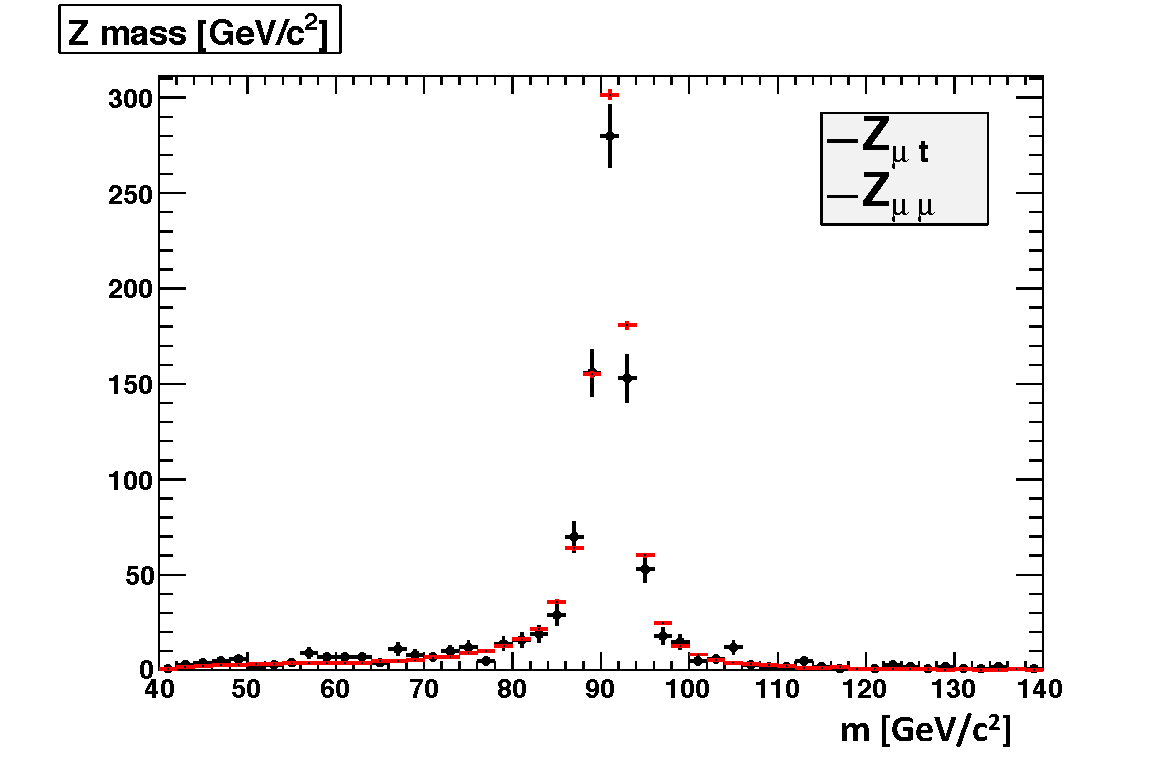
\includegraphics{FifthChapter/comparison_mm_mt_lin_rebin.pdf}}
      \end{center}
    \end{minipage}
%\vspace{0.5cm}
     \begin{minipage}{73mm}
       \begin{center}
       \resizebox{!}{0.75\textwidth}{
       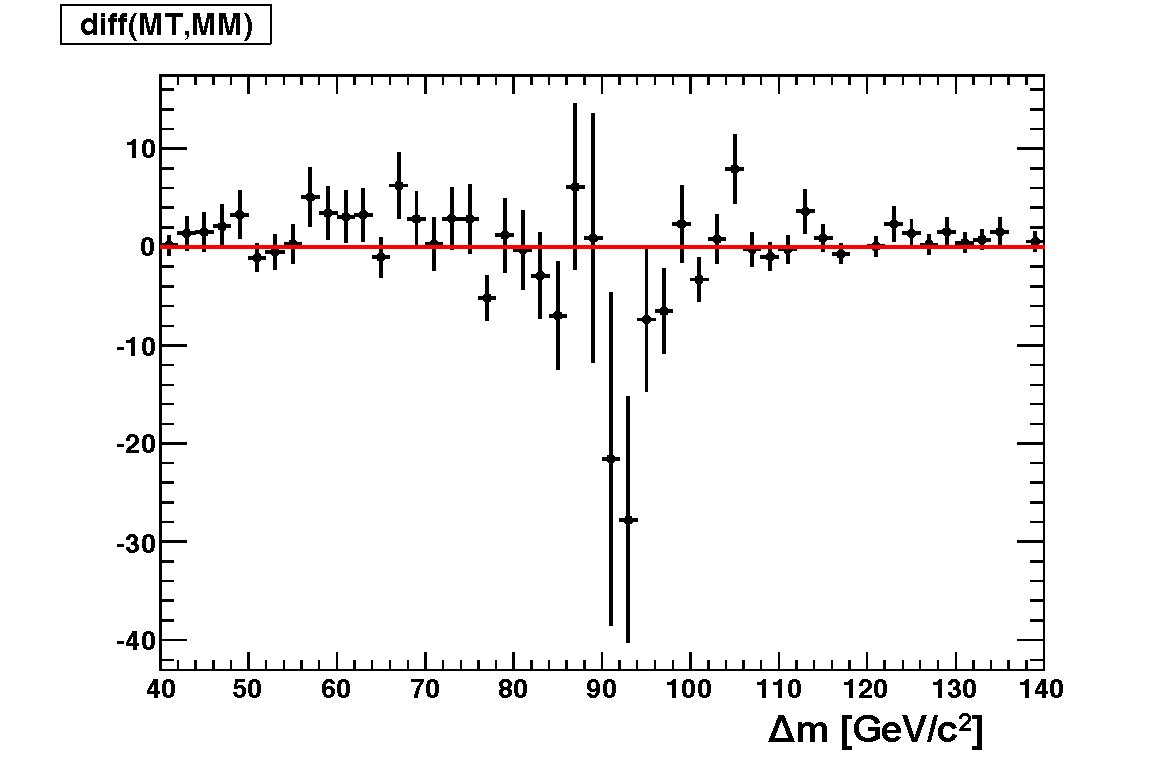
\includegraphics{FifthChapter/comparison_mm_mt_diff_rebin.pdf}
       }
       \end{center}
    \end{minipage}
\caption{Left: invariant mass distribution for selected $\Zmumu$ (red points) and $\Zmut$ (black 
points) candidates in signal events. The $\Zmumu$ distribution is normalized in order to have the 
same number of events as the $\Zmut$ sample. Right: difference between the $\Zmumu$ and $\Zmut$ 
distributions.}
\label{fig:mmVsmtComparison}
\end{figure}      

\begin{figure}[hbtp]
   \begin{minipage}{73mm}
      \begin{center}
      \resizebox{!}{0.75\textwidth}{
  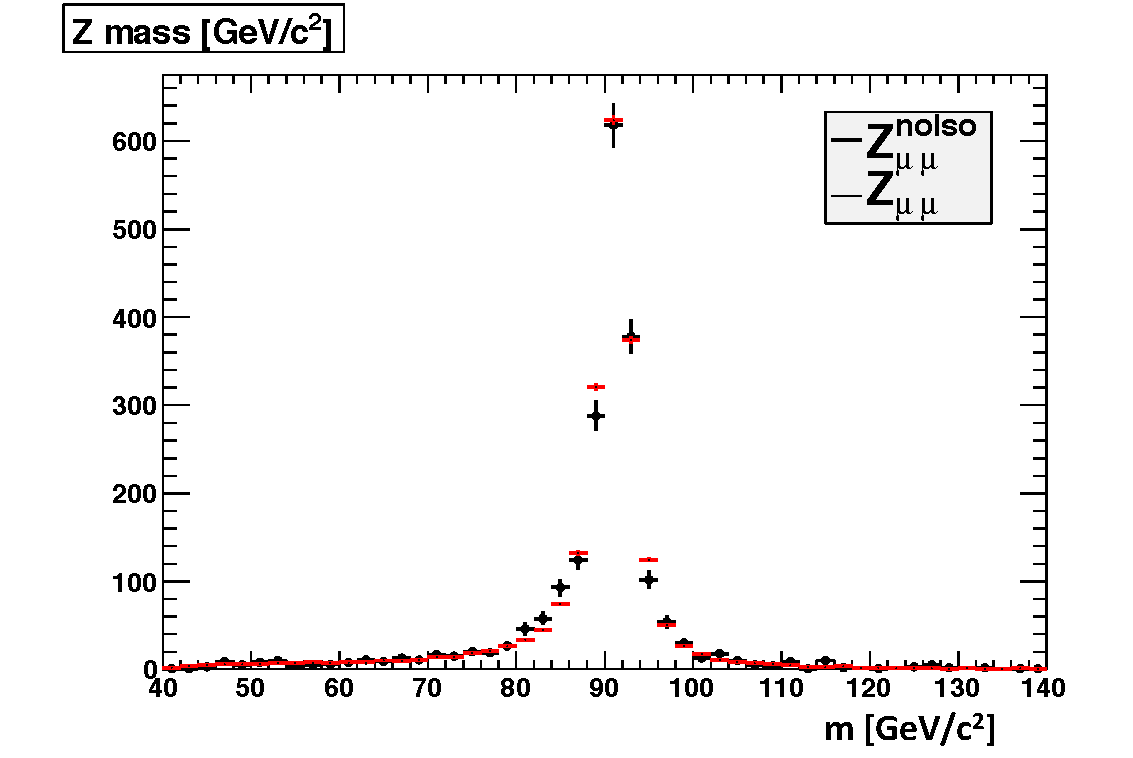
\includegraphics{FifthChapter/comparison_mm_notiso_lin_rebin.pdf}
       }
      \end{center}
    \end{minipage}
    \begin{minipage}{73mm}
       \begin{center}
       \resizebox{!}{0.75\textwidth}{
       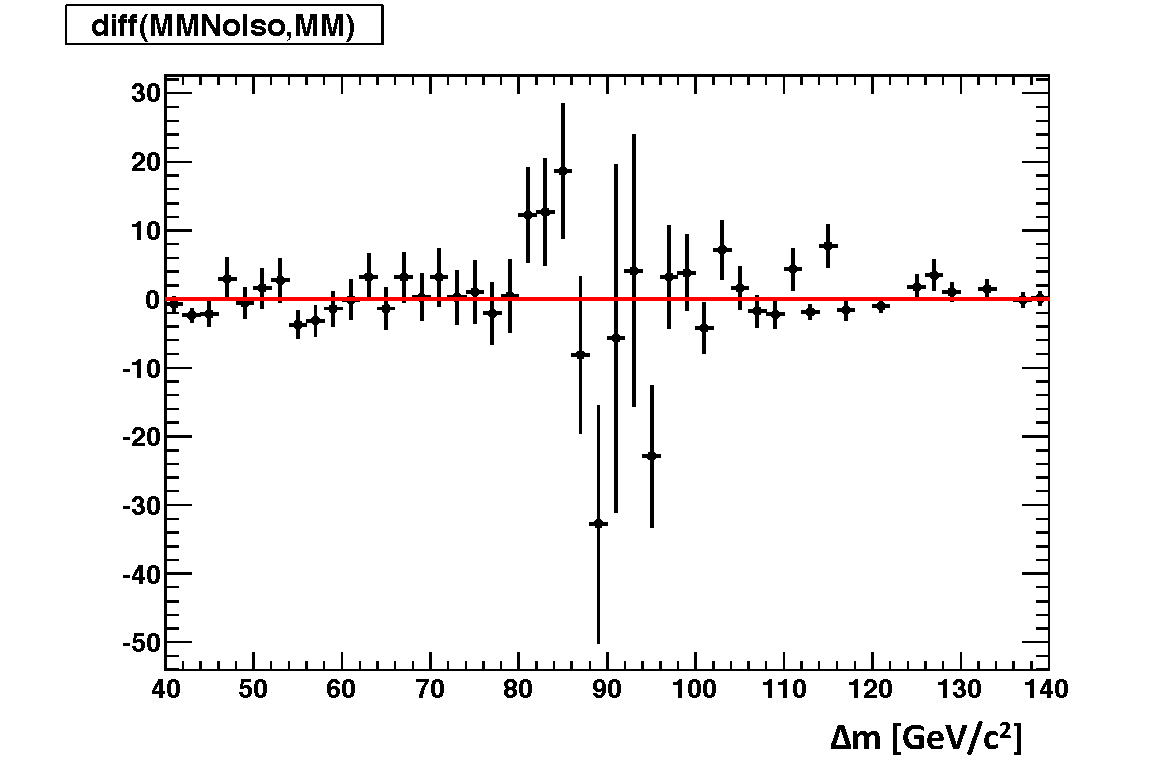
\includegraphics{FifthChapter/comparison_mm_notiso_diff_rebin.pdf}
       }
       \end{center}
    \end{minipage}
\caption{Left: invariant mass distribution for selected $\Zmumu$ (red points) and $\ZmumuNonIso$ (black 
points) candidates in signal events. The $\Zmumu$ distribution is normalized in order to have the 
same number of events as the $\ZmumuNonIso$ sample. Right: difference between the $\Zmumu$ and $\ZmumuNonIso$ 
distributions.}
\label{fig:mmVsmmNoIsoComparison}
\end{figure}      

We have also assumed that the isolation efficiency is identical for
global muons, tracks and stand-alone muons. For the latter, in particular,
the worse direction resolution could produce a slightly different
isolation efficiency. We measured on the Monte Carlo signal sample that 
the difference in isolation efficiency is very small, and compatible with
zero within errors: 
\begin{displaymath}
\effIso^{\mathrm{s.a.}}-\effIso^{\mathrm{glob.}}=0.007\pm0.057\%\,\,.
\end{displaymath}

%With an optimized combined tracker plus calorimeter isolation, described in 
%Section~\ref{isolation}, which has an efficiency closer to unity, 
%we obtain similar results:
%\begin{displaymath}
%\effIso^{\mathrm{s.a.}}-\effIso^{\mathrm{glob.}}=0.010\pm0.036\%\,\,.
%\end{displaymath}

In order to determine from data a model for the PDF of 
the peak function for the $\Zmus$ category, $f_{peak}^{s}(m)$, 
we consider the $\Zmumu$ candidates, and for one of the muons
we take the momentum measured from the muon detector track fit only,
in order to mimic a stand-alone muon. We avoid to put the same event
twice in the histogram, by choosing alternatively the first (second)
muon for even (odd) events respectively.
This makes the signal shape description entirely data-driven. Figure~\ref{fig:ZMuS_PdfComparison} compares the
invariant mass distribution of the selected $\Zmus$ candidates
with the shape obtained from $\Zmumu$ candidates.

\begin{figure}[hbtp]
    \begin{minipage}{73mm}
      \begin{center}
\resizebox{1.15\textwidth}{!}{{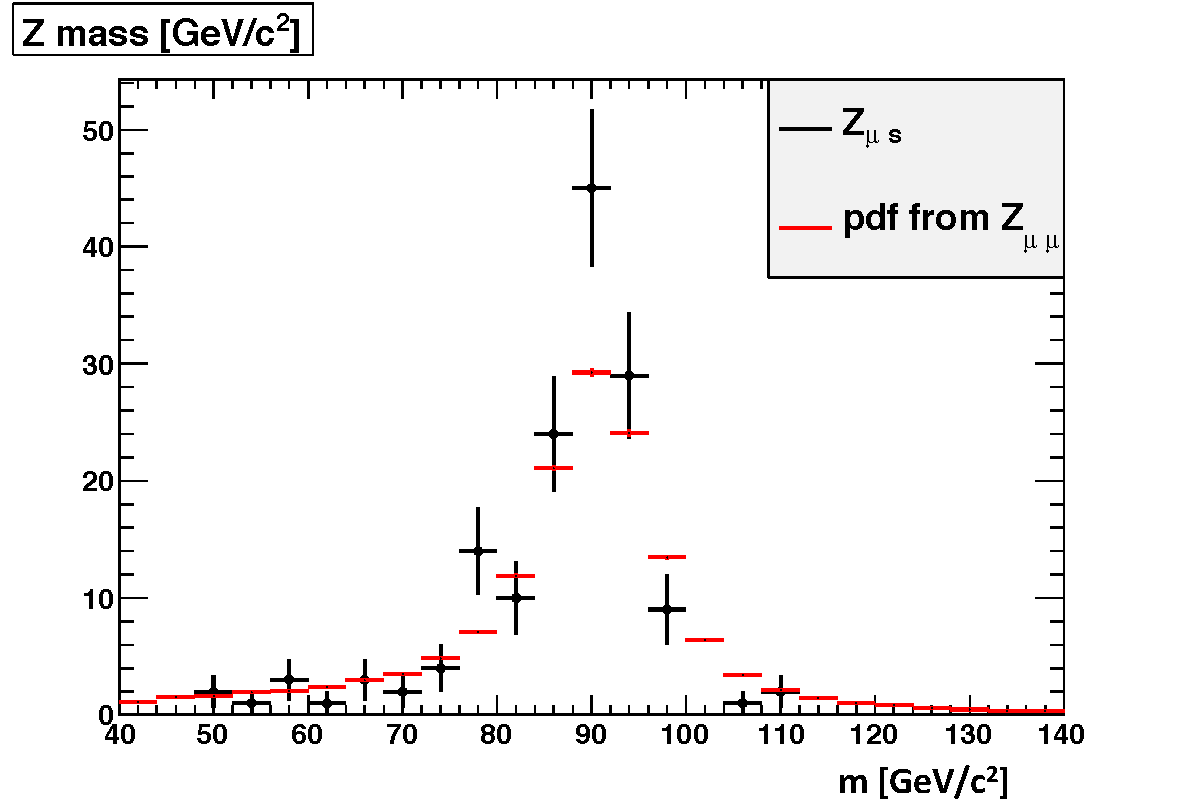
\includegraphics{FifthChapter/comparison_pdfms_ms_lin_rebin.pdf}}}
      \end{center}
    \end{minipage}
    \begin{minipage}{73mm}
       \begin{center}
       \resizebox{!}{0.75\textwidth}{
       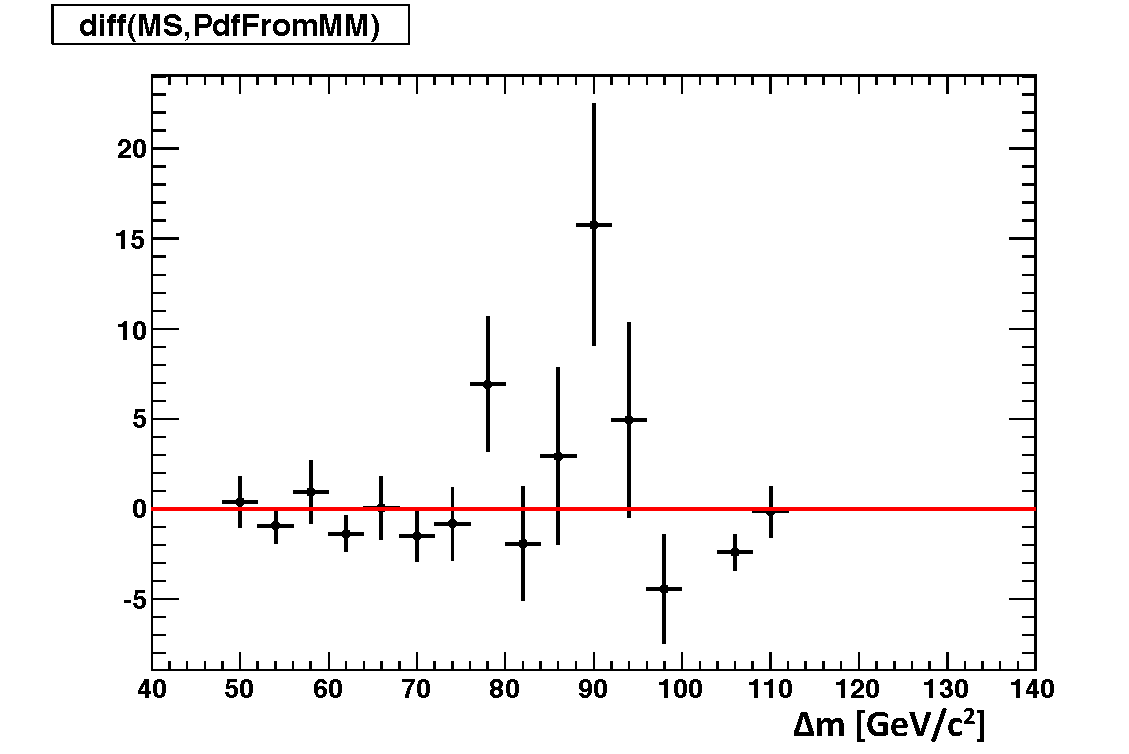
\includegraphics{FifthChapter/comparison_pdfms_ms_diff_rebin.pdf}
     }
      \end{center}
    \end{minipage}
\caption{Left: invariant mass distribution for selected $\Zmus$ candidates in signal events
(black points) superimposed to the pdf (red points) determined from $\Zmumu$ candidates by using, for
one of the muons in the pair, the momentum of the associated stand-alone muon.}
\label{fig:ZMuS_PdfComparison}
\end{figure}      

Background functions are modeled as products of exponential terms with polynomials 
of different order for the three samples for which the background is not neglected:
\begin{eqnarray}
  b_{\mu t}(m) & = & N^b_{\mu t} (1 + a_1 m + a_2 m^2) e^{-\alpha m} \\
  b_{\mu\mu}^{\mathrm{non\,iso}}(m) & = & N_{\mu\mu}^{b\,\,{\mathrm{non\,iso}}} (1 + b_1 m) e^{-\beta m} \\
  b_{\mu s}(m) & = & N^b_{\mu s} e^{-\gamma m} 
\end{eqnarray}
%  f_{peak}^{s}(m) & = & \frac{1}{\sqrt{2\pi\sigma_s^2}} e^{-\frac{(m - M)^2}{2 \sigma_s^2} } \\
%The peak function for the $\Zmus$ category, $f_{peak}^{s}(m)$, is modelled as a
%Gaussian, due to the poor resolution, and the low statistics in that sample:
With the binned mass values of the five di-muon categories we performe a Poisson likelihood ratio fit\cite{PLR}, minimizing the function:
\begin{equation}
R = -2 \ln{\lambda(m)} =  -2 \ln{\frac{\mathrm{Poisson}(n_i,
    \nu_i)}{\mathrm{Poisson}(n_i, n_i)}}
%\sum_{i=1,...5} \chi^2_{\lambda,i}
\end{equation}
where $\nu_i$ is the expected number of events in the i-bin of the
mass histograms and $n_i$ is the measured number of events.
For independent Poisson distribution $n_i$ one can demonstrates that
that it is equivalent to minimize:
\begin{equation}
R =  \sum_{i=1,...5} \chi^2_{\lambda,i}   = 2 \sum_{i=i,....,nBins} \nu_i - n_{i} + n_i \log{\frac{n_i}{\nu_i}} 
\end{equation}

A benefit of this statistic technique is that it allows a
goodness-of-fit test, as for sufficiently large $\nu_i$ the minimum of $R$ follows a $\chi^2$ distribution.

So, starting from the 5 independent di-muon categories, the unknown best fit parameters are obtained by minimizing:
\begin{eqnarray*} \label{chi2}
R & = &  
\frac{(\NmumuTwoHlt - \NZtomumu\effHlt^2\effIso^2\effTrk^2\effSa^2)^2}{\NmumuTwoHlt} +  \\
& & \frac{(\NmumuOneHlt - 2\NZtomumu\effHlt(1-\effHlt)\effIso^2\effTrk^2\effSa^2)^2}{\NmumuOneHlt} +  \\
& & \chi^2_{\lambda, \mu s} + 
\chi^2_{\lambda, \mu t} + 
\chi^{\nonIso\,\, 2}_{\lambda, \mumu}\, , 
\end{eqnarray*} 
where we count the events $\ZmumuOneHlt$ and $\ZmumuTwoHlt$ golden
categories and $\chi^2_{\lambda, \mu s}$, $\chi^2_{\lambda, \mu t}$ and
$\chi^{\nonIso\,\, 2}_{\lambda, , \mumu}$ are the
Poisson likelihood ratio of the di-muon mass binned histograms for the
three categories $\Zmus$, $\Zmut$, and $\ZmumuNonIso$. This technique
corrects histograms with 0 entries bin and reduce possible biases with
low statistics. The likelihood ration becomes
equivalent to simple $\chi^2$ for enough statistics and gives the same
statistical errors.


We perform the fit in the range $60 < m < 120~\mathrm{GeV}/c^2$.



\subsection{Correlation studies}
\label{correlationStudies}
In the following sub-sections we consider the possible
effect of:
\begin{itemize}
\item kinematic correlation between the two muons
\item correlation of muon detector reconstruction and HLT efficiency
  distributions as functions of $\eta$ and $p_T$ 
\item correlation of tracker reconstruction and isolation efficiency distributions
\end{itemize}

\subsubsection{Efficiency correlation between the two muons}

In the above fit model we assumed that we can factorize
the efficiency terms for the two muons (that are products
of reconstruction, isolation and trigger efficiencies).
We now justify this assumptions, that consists in neglecting
the correlation of the efficiency terms, and provide a method 
to estimate the uncertainty caused by this assumption.

The differential $Z$ yield, 
as a function of the two muon three-momenta, can be written 
as:
\begin{equation}
\frac{\mathrm{d}^3n^0}{\mathrm{d}^3p_1 \mathrm{d}^3p_2} = N^0 f_0 (\vec{p_1}, \vec{p_2}) \times \epsilon_1(\vec{p_1})\epsilon_2(\vec{p_2})\,\, ,
\end{equation}
where $N^0$ is the total number of produced events, $\vec{p_1}$ and $\vec{p_2}$ are
the two muons three-momenta, $f_0(\vec{p_1}, \vec{p_2})$ is the probability density function
that takes into account the process matrix element, phase space, and detector resolutions.
We introduce the efficiency terms for the two muons as: 
$\epsilon_1(\vec{p_1})$, $\epsilon_2(\vec{p_2})$, whose 
interpretation varies for the different samples we consider.
In the case of the sample reconstructed as a pair of global muons, for instance,
the two functions $\epsilon_1$ and $\epsilon_2$ coincide, and are equal
to the product $\effTrk(\vec{p})\effSa(\vec{p})\effIso(\vec{p})\effHlt(\vec{p})$. 


The differential $Z$ yield as a function of the muon pair invariant mass is:


\begin{equation}
\label{eq:densityWithEfficiency}
\frac{\mathrm{d}n}{\mathrm{d} m} = N_0 \int \mathrm{d}^3p_1 \mathrm{d}^3p_2 f_0(\vec{p_1}, \vec{p_2}) \delta(m_{12}(\vec{p_1}, \vec{p_2}) - m) \epsilon_1(\vec{p_1}) \epsilon_2(\vec{p_2})\,\,\ ,
\end{equation}
or sum of similar terms with different $\epsilon_1(\vec{p_1})$ and $\epsilon_2(\vec{p_2})$. The efficiency terms 
for the other 
categories are reported in Table~\ref{tab:effTerms} for
completeness. In the above equation $m_{12}$ is the
di-muon invariant mass, which can be writtem as  $m_{12} = (\vec{p_1}, \vec{p_2}) = 2 p_1 p_2 ( 1 - \cos \theta_{12})$ neglecting the muon mass.


\begin{equation}
\label{diffN0}
\frac{\mathrm{d}n^0}{\mathrm{d} m} = N_0 \int \mathrm{d}^3p_1 \mathrm{d}^3p_2 f_0(\vec{p_1}, \vec{p_2}) \delta(m_
{12}(\vec{p_1}, \vec{p_2}) - m)\,\,\ ,
\end{equation}



\begin{table}[htbp]
\vspace{0.5cm}
\begin{center}
{\footnotesize
\begin{tabular}{|l|c|c|}
\hline
Category & $\epsilon_1(\vec{p_1})$ & $\epsilon_2(\vec{p_2})$ \\
\hline\hline
$\ZmumuTwoHlt$ & $\effTrk(\vec{p_1})\effSa(\vec{p_1})\effIso(\vec{p_1})\effHlt(\vec{p_1})$ & $\effTrk(\vec{p_2})\effSa(\vec{p_2})\effIso(\vec{p_2})\effHlt(\vec{p_2})$ \\
\hline
$\ZmumuOneHlt$ & $\effTrk(\vec{p_1})\effSa(\vec{p_1})\effIso(\vec{p_1})\effHlt(\vec{p_1})$  & $\effTrk(\vec{p_2})
\effSa(\vec{p_2})\effIso(\vec{p_2})(1-\effHlt(\vec{p_2}))$ \\
 & $\effTrk(\vec{p_1})\effSa(\vec{p_1})\effIso(\vec{p_1})(1-\effHlt(\vec{p_1}))$  & $\effTrk(\vec{p_2})\effSa(\vec{p_2})\effIso(\vec{p_2})\effHlt(\vec{p_2})$ \\
\hline
$\Zmus$ & $\effTrk(\vec{p_1})\effSa(\vec{p_1})\effIso(\vec{p_1})\effHlt(\vec{p_1})$ & $(1-\effTrk(\vec{p_2}))\effSa(\vec{p_2})\effIso(\vec{p_2})$ \\
       &  $(1-\effTrk(\vec{p_1}))\effSa(\vec{p_1})\effIso(\vec{p_1})$ & $\effTrk(\vec{p_2})\effSa(\vec{p_2})\effIso(\vec{p_2})\effHlt(\vec{p_2})$ \\
\hline
$\Zmut$ & $\effTrk(\vec{p_1})\effSa(\vec{p_1})\effIso(\vec{p_1})\effHlt(\vec{p_1})$ & $\effTrk(\vec{p_2})(1-\effSa(\vec{p_2}))\effIso(\vec{p_2})$ \\
       &  $\effTrk(\vec{p_1})(1-\effSa(\vec{p_1}))\effIso(\vec{p_1})$ & $\effTrk(\vec{p_2})\effSa(\vec{p_2})\effIso(\vec{p_2})\effHlt(\vec{p_2})$ \\
\hline
$\ZmumuNonIso$ & $\effTrk(\vec{p_1})\effSa(\vec{p_1})\effIso(\vec{p_1})\effHlt(\vec{p_1})$ & $\effTrk(\vec{p_2})\effSa(\vec{p_2})(1-\effIso(\vec{p_2}))\effHlt(\vec{p_2})$ \\
      & $\effTrk(\vec{p_1})\effSa(\vec{p_1})(1-\effIso(\vec{p_1}))\effHlt(\vec{p_1})$ & $\effTrk(\vec{p_2})\effSa(\vec{p_2})\effIso(\vec{p_2})\effHlt(\vec{p_2})$ \\
      & $\effTrk(\vec{p_1})\effSa(\vec{p_1})(1-\effIso(\vec{p_1}))\effHlt(\vec{p_1})$ & $\effTrk(\vec{p_2})\effSa(\vec{p_2})(1-\effIso(\vec{p_2}))\effHlt(\vec{p_2})$ \\
      & $\effTrk(\vec{p_1})\effSa(\vec{p_1})\effIso(\vec{p_1})\effHlt(\vec{p_1})$ & $\effTrk(\vec{p_2})\effSa(\vec{p_2})(1-\effIso(\vec{p_2}))\effHlt(\vec{p_2})$ \\
      & $\effTrk(\vec{p_1})\effSa(\vec{p_1})(1-\effIso(\vec{p_1}))\effHlt(\vec{p_1})$ & $\effTrk(\vec{p_2})\effSa(\vec{p_2})\effIso(\vec{p_2})(1-\effHlt(\vec{p_2}))$ \\
      & $\effTrk(\vec{p_1})\effSa(\vec{p_1})(1-\effIso(\vec{p_1}))\effHlt(\vec{p_1})$ & $\effTrk(\vec{p_2})\effSa(\vec{p_2})(1-\effIso(\vec{p_2}))(1-\effHlt(\vec{p_2}))$ \\
      & $\effTrk(\vec{p_1})\effSa(\vec{p_1})\effIso(\vec{p_1})(1-\effHlt(\vec{p_1}))$ & $\effTrk(\vec{p_2})\effSa(\vec{p_2})(1-\effIso(\vec{p_2}))\effHlt(\vec{p_2})$ \\
      & $\effTrk(\vec{p_1})\effSa(\vec{p_1})(1-\effIso(\vec{p_1}))(1-\effHlt(\vec{p_1}))$ & $\effTrk(\vec{p_2})\effSa(\vec{p_2})\effIso(\vec{p_2})\effHlt(\vec{p_2})$ \\
      & $\effTrk(\vec{p_1})\effSa(\vec{p_1})(1-\effIso(\vec{p_1}))(1-\effHlt(\vec{p_1}))$ & $\effTrk(\vec{p_2})\effSa(\vec{p_2})(1-\effIso(\vec{p_2}))\effHlt(\vec{p_2})$ \\
\hline
\end{tabular}
}
\end{center}
\caption{List of the efficiency terms to be used in Equation (\ref{eq:densityWithEfficiency}) for the different r
reconstructed $Z$ categories.}
\label{tab:effTerms}
\end{table}

In the fit model above we made the approximation that the efficiency terms
can be factorized as average terms $\bar{\epsilon_1}$, $\bar{\epsilon_2}$:
\begin{equation}
\frac{\mathrm{d}n}{\mathrm{d} m} \simeq \frac{\mathrm{d}n^\prime}{\mathrm{d} m} = N_0 \bar{\epsilon_1} \bar{\epsilon_2} \int \mathrm{d}^3p_1 \mathrm{d}^3p_2 f_0(\vec{p_1}, \vec{p_2}) \delta(m_{12}(\vec{p_1}, \vec{p_2}) - m)\,\
,\ .
\end{equation}
where:
\begin{eqnarray}
\label{averageEff}
\bar{\epsilon_1} & = & \langle \epsilon_1(\vec{p_1}) \rangle = \int \mathrm{d}^3p_1 \mathrm{d}^3p_2 f_0(\vec{p_1}
, \vec{p_2}) \epsilon_1(\vec{p_1})\,\, , \\
\bar{\epsilon_2} & = & \langle \epsilon_2(\vec{p_2}) \rangle = \int \mathrm{d}^3p_1 \mathrm{d}^3p_2 f_0(\vec{p_1}
, \vec{p_2}) \epsilon_2(\vec{p_2})\,\, .
\end{eqnarray}

The difference between the approximated and exact expressions,
due to the normalization of $f(\vec{p_1}, \vec{p_2})$:
\begin{equation}
\int \mathrm{d}^3p_1 \mathrm{d}^3p_2 f_0(\vec{p_1}, \vec{p_2}) = 1\,\, 
\end{equation}
is:
\begin{equation}
\frac{\mathrm{d}n}{\mathrm{d} m} - \frac{\mathrm{d}n^\prime}{\mathrm{d} m} =
 N_0 \int \mathrm{d}^3p_1 \mathrm{d}^3p_2 f_0(\vec{p_1}, \vec{p_2}) \delta(m_{12}(\vec{p_1}, \vec{p_2}) - m) (\epsilon_1(\vec{p_1}) \epsilon_2(\vec{p_2}) - \bar{\epsilon_1}\bar{\epsilon_2})\,\, .
\end{equation}

Integrating over the mass $m$, in order to extract the cross-section, in a range $[m_1, m_2]$, one has:
\begin{eqnarray}
N & = & \int_{m_1}^{m_2} \mathrm{d}m \frac{\mathrm{d}n}{\mathrm{d} m}\,\, ,\\
N^\prime & = & \int_{m_1}^{m_2} \mathrm{d}m \frac{\mathrm{d}n^\prime}{\mathrm{d} m}\,\, ,
\end{eqnarray}
hence:
\begin{eqnarray*}
N - N^\prime & = & N_0 \int \mathrm{d}^3p_1 \mathrm{d}^3p_2f_0(\vec{p_1}, \vec{p_2})(\epsilon_1(\vec{p_1})\epsilon_2(\vec{p_2}) -\bar{\epsilon_1}\bar{\epsilon_2}) \\
 & = & N_0 \langle \epsilon_1(\vec{p_1})\epsilon_2(\vec{p_2}) -\bar{\epsilon_1}\bar{\epsilon_2} \rangle \\
 & = & N_0 \langle (\epsilon_1(\vec{p_1}) -\bar{\epsilon_1})(\epsilon_2(\vec{p_2})-\bar{\epsilon_2}) \rangle \\
 & = & N_0 \mathrm{cov}(\epsilon_1(\vec{p_1}), \epsilon_2(\vec{p_2})) \equiv N_0 \mathrm{cov}_{12}\,\, ,
\end{eqnarray*}
or equivalently:
\begin{equation}
\frac{N - N^\prime}{N_0} = \frac{\Delta N}{N_0} = \mathrm{cov}(\epsilon_1(\vec{p_1}), \epsilon_2(\vec{p_2}))\,\, 
.
\end{equation}

So, the assumption we made is equivalent to neglect the correlation term between
the two muon efficiencies, $\mathrm{cov}_{12}$.

Note that the above term is quadratic in the statistical dispersion of the efficiencies in the
$p_t$ and $\eta$ range considered.   So, taking two efficiencies for
the table \ref{tab:effTerms}, if we assume that $\epsilon_k(\vec{p_k}) -\bar{\epsilon_k}$
($k = 1, 2$) is at most $\delta$, the relative systematic error introduced by the
approximation will be smaller then $\delta^2$. This would give a first way to estimate an upper
limit to this systematic effect just looking at the efficiency excursion in 
the efficiency tables obtained with other method such as the
``Tag and Probe'' (see Section \ref{TriggerZmumu} for an
explanation of this method) : a 10\% dispersion would give a 1\% effect.

A more precise way to estimate this effect could be done using the  T\&P efficiency
tables $(\epsilon_k^{tp}(\vec{p}))$. We could estimate the needed terms as discrete 
averages over the signal sample:
\begin{equation}
\bar{\epsilon}_k^{tp} = \frac{1}{N_\mathrm{obs}^{\mu,\, k}}\sum_{i=1, \ldots n}^{N_\mathrm{obs}^{\mu,\, k}} \epsilon_k^{tp}(\vec{p_i})\,\,, \,\, k = 1,2 \,\, ,
\end{equation}
and:
\begin{eqnarray}
\mathrm{cov}_{12}^{tp} & = &\frac{1}{N_\mathrm{obs}^Z}\sum_{i=1, \ldots n}^{N_\mathrm{obs}^Z} (\epsilon_1^{tp}(\vec{p_{1(i)}}) - \bar{\epsilon}_1^{tp})(\epsilon_2^{tp}(\vec{p_{2(i)}}) - \bar{\epsilon}_2^{tp}) \\
  & = & \frac{1}{N_\mathrm{obs}^Z}\sum_{i=1, \ldots n}^{N_\mathrm{obs}^Z} \epsilon_1^{tp}(\vec{p_{1(i)}})\epsilon_2^{tp}(\vec{p_{2(i)}}) - \bar{\epsilon}_1^{tp}\bar{\epsilon}_2^{tp}\,\, . \label{cov12}
\end{eqnarray}

Above, $N_\mathrm{obs}^Z$ is the number of observed $Z$ events and
is the number of observed muons in $Z$ events for the two category $k=1,\, 2$
or for the unique category, in case of $Z$ reconstructed from a pair of global muons. 

Studies based on MC samples demonstrated that
the correlation effect can be neglected at the 0.01\% level.

\subsubsection{Correlation between trigger efficiency and Reconstruction efficiency}
\label{muhltcorrelation}
In this section we discuss the correlation between trigger and reconstruction efficiency. 
This correlation cannot be neglected a-priori and brings to the definition of an effective 
average trigger efficiency.
The trigger efficiency we are considering is indeed the product
of the efficiencies L1, L2 and L3 trigger event selection paths. 

We rewrite Equation~(\ref{averageEff}) as follows:

\begin{equation}
\bar{\epsilon_i}  = \langle \epsilon_i(\vec{p_i}) \rangle = \int \mathrm{d}^3p_1 \mathrm{d}^3p_2 f_0(\vec{p_1}, \vec{p_2}) \epsilon_i(\vec{p_i})\,\, ,i = 1, 2\,\, ,
\end{equation}
where $\epsilon_i(\vec{p_i})$, $i=1,2$, is one of the terms listed in Table~\ref{tab:effTerms}.
We define for simplicity, omitting the subscript $i$:

\begin{equation}
\bar{\epsilon}  = \langle \epsilon(\vec{p}) \rangle = \int \mathrm{d}^3p f_0(\vec{p}) \epsilon(\vec{p})\,\, ,
\end{equation}

where, for $i=1$, $f_0(\vec{p_1}) = \int \mathrm{d}^3p_2 f_0(\vec{p_1}, \vec{p_2})$, and similarly
for $i=2$, $f_0(\vec{p_2}) = \int \mathrm{d}^3p_1 f_0(\vec{p_1}, \vec{p_2})$.

In the case of the sample reconstructed as a pair of global muons, for instance,
the average:
\begin{equation}
 \bar{\epsilon} = \langle \effTrk(\vec{p})\effSa(\vec{p})\effIso(\vec{p})\effHlt(\vec{p}) \rangle
\end{equation}
does not coincide with the product of the averages: 
$\langle\effTrk(\vec{p})\rangle\langle\effSa(\vec{p})\rangle\langle\effIso(\vec{p})\rangle\langle\effHlt(\vec{p})
\rangle$, and again we can assume factorization
wherever correlation terms can be neglected. It is reasonable to assume that
$\effIso(\vec{p})$ and $\effTrk(\vec{p})$ are uncorrelated w.r.t. the other terms while
it could be not the case for $\effSa(\vec{p})$ and
$\effHlt(\vec{p})$, which can be correlated, since single muon trigger
is very related to the geometry of the muon detector.

When we express the differential $Z$ yields of the different categories, we have, for each of
the two muons, efficiency terms that contain $\effSa(\vec{p})$ and $\effHlt(\vec{p})$
either as products $\effSa(\vec{p})\cdot\effHlt(\vec{p})$, or as single terms containing just $\effSa(\vec{p})$.
We never find single terms in $\effHlt(\vec{p})$. Thus, 
when we compute the average terms,
we are still allowed to use factorization in Equations~(\ref{eqNmumuTwoHlt}),
(\ref{eqNmumuOneHlt}), (\ref{eqNmus}), (\ref{eqNmut}) and (\ref{eqNmumuNonIso}), 
but we have to re-define $\effHlt$ as:
\begin{equation}
\label{eq:effHltRatio}
\effHlt = \frac{\langle\effSa(\vec{p})\cdot\effHlt(\vec{p})\rangle}{\langle\effSa(\vec{p})\rangle}\,\, ,
\end{equation}
and so we interprete $\effHlt$ as the efficiency to trigger a muon
which has been correctly reconstructed in the muon system. 

\subsubsection{Correlation between tracking efficiency and isolation efficiency}
A correlation between tracking efficiency and isolation efficiency may
occour in case of very bad tracker noise or large event pile-up situation,
in which a simultaneous loss of tracker efficiency and isolation power
generated by excess of noise in some detector regions could be present.

If we don't neglect this correlation, a similar treatment as it was
discussed in Section~\ref{muhltcorrelation} can be done. In a similar way,
we can re-define an ``effective'' isolation efficiency, similarly
to Eq.~(\ref{eq:effHltRatio}):
\begin{equation}
\label{eq:effIsoRatio}
\effIso = \frac{\langle\effTrk(\vec{p})\cdot\effIso(\vec{p})\rangle}{\langle\effTrk(\vec{p})\rangle}\,\, ,
\end{equation}
interpreting $\effIso$ as the efficiency of the isolation cut on muon
fully reconstructed  in the tracking system.
All efficiency terms in the definition of $Z$ categories from Equations~(\ref{eqNmumuTwoHlt}),
(\ref{eqNmumuOneHlt}), (\ref{eqNmut}) and (\ref{eqNmumuNonIso}) remain 
unchanged, but correlation must be taken into account in 
the efficiency term of the $\Zmus$ category, in Equation (\ref{eqNmus}).
The term, including correlation, is:

\begin{eqnarray*}
\langle \effTrk(\vec{p_1})\effIso(\vec{p_1})(1-\effTrk(\vec{p_2}))\effIso(\vec{p_2})\rangle + \\
\langle (1-\effTrk(\vec{p_1}))\effIso(\vec{p_1})\effTrk(\vec{p_2})\effIso(\vec{p_2})\rangle = \\
2\langle \effTrk\effIso\rangle(\langle\effIso\rangle-\langle\effTrk\effIso\rangle)\,\,.
\end{eqnarray*}
Replacing in the above term:
\begin{displaymath}
\langle\effTrk\effIso\rangle = \effTrk\effIso
\end{displaymath}
\begin{displaymath}
\langle\effIso\rangle = \effIso - \frac{\mathrm{cov}_{trk\,\mathrm{iso}}}{\effTrk} = \effIso\left(1-\frac{\mathrm
{cov}_{trk\,\mathrm{iso}}}{\effTrk\effIso}\right)\,\,.
\end{displaymath}
We can corrected Equations~(\ref{eqNmus}) including a possible correlation term:
\begin{equation}
\Nmus = 2 \NZtomumu \effHlt \effIso^2 \effTrk \effSa^2 \left( (1 - \effTrk) - \frac{\mathrm{cov}_{trk\,\mathrm{is
o}}}{\effTrk\effIso}\right)\,\,.
\end{equation}

This correction would only affect the $\Zmus$ category that is used to determine the 
tracker efficiency which we expect that, under normal detector operation, would
be very close to one. So, we expect this category to be the one with the smallest
statistics. A deviation of the number of $\Zmus$ events would result 
in a corresponding variation on the tracker inefficiency $(1-\effTrk)$, that would
result in a much smaller relative variation of $\effTrk$, being $\effTrk$ close to the unity.

If this covariance term would turn out to be significantly different from zero,
as alternative, we can drop the isolation request to the stand-alone muon, and
this will allow to fully absorb the covariance term into the redefinition
of $\effIso$, as done in Section~\ref{muhltcorrelation} for $\effHlt$.

Tracker background and event pile-up don't have such a serious impact, especially
at low luminosity, to impair dramatically the tracker performance, as
in the case of the current measurement described in this work. Anyway, in order
to estimate correctly the correlation term under those pessimistic conditions, a realistic
estimate would need either a proper simulation of those detector and run conditions, or control 
samples from real data taken under those conditions. It's important to note that the same effect
may also affect othe $\ZmumuTwoHlt$ r currently used methods to estimate detector efficiencies, such as
the Tag and Probe method (see Section \ref{TriggerZmumu}).


\subsection{Data samples}
The 2010 7 TeV collision data sample used for this
analysis (Run2010A) amounts  to an integrated luminosity of 2.9
pb$^{-1}$ (see \ref{sec:LumiFromZ} for details on how the
luminoisty measurement is done in CMS).
We have used the following Monte Carlo samples generated
with the standard CMS generator,
simulation and reconstruction chain, assuming a center of mass energy of $\sqrt{s} = 7~\mathrm{TeV}$ 
with the same detector condition and reconstruction parameter used
for the data taking:
\begin{itemize}
\item $pp\rightarrow Z/\gamma^{\ast} X\rightarrow \mu^+\mu^- X$
\item $pp\rightarrow W^\pm X\rightarrow \mu^\pm\nu_{\mu} X$
\item QCD jets events containing
at least one muon with $p_t > 15 \mathrm{GeV}/c$ 
\item $t\bar{t}$.
\item $WZ$ and $WW$
\end{itemize}

The number of events for each MC sample, the product of the NLO cross-section ($\sigma$) 
times the generator kinematic filter efficiency
($\epsilon_{\mathrm{filter}}$, i.e. the fraction of generated event
witch fall effectively in the kineatic region accessible by the detectors), and the equivalent
integrated luminosity ($\int\mathcal{L}\mathrm{d}t$) are shown in
Table~\ref{datasamples}. 

\begin{table}[htbp]
\centering
\begin{tabular}{|l|r|r|r|}
\hline
Sample &  $\sigma\times\epsilon_{\mathrm{filter}}$ (pb) & $\int\mathcal{L}\mathrm{d}t$ (pb$^{-1}$)\\
\hline\hline
$pp\rightarrow Z X \rightarrow\mu^+\mu^-  X (m>20)$ & 1686  & 100  \\
$pp\rightarrow W^+ X \rightarrow\mu^+ \nu_{\mu} X  $  & 6152  &100 \\
$pp\rightarrow W^- X \rightarrow\mu^- \nu_{\mu} X $  & 4179 &100 \\
QCD jets, muon $p_t > 15$~$\mathrm{GeV}/c$ & 79688 & 60   \\
$t\bar{t}$ & 162 & 100 \\
$pp\rightarrow Z X \rightarrow\tau^+\tau^- X$ & 1686 &  100 \\
$W Z $ & 43 &  537 \\
$WW$ & 18 &  100 \\
$ZZ$ & 5.9 &  100 \\
\hline
\end{tabular}
\caption{Analyzed MC data samples.}
\label{datasamples}
\end{table}

The analyzed samples are first processed through a preselection phase
denominated ``skimming'' where HLT requirements are applied. 
At skimming level, it is also required the presence of at least two
reconstructed muons or one muon plus one tracker track, with $p_T > 15
\mathrm{GeV/c}$.
After that, in order to further reduce the data samples, a secondary skim (sub-skim) was
run and the a very light  output was has been produced.

\subsection{Event selection}
Events are required to satisfy the single non-isolated muon trigger 
with a (L3 trigger step) $p_T$ cut of 9 GeV (7 GeV at L1 trigger step) .

Muons used for $Z$ reconstruction are checked for matching with
an HLT object (see Sect.~\ref{TriggerZmumu} for the HLT matching requirement
used in the different samples of $Z$ candidates and for additional
muon trigger efficiencies estimation results with $\Zmumu$).


We require that both muon candidates, either global or stand-alone muons, or tracker tracks,
must satisfy:
\begin{displaymath}
p_T > 20~\mathrm{GeV}/c\,\, , \mathrm{and} \:\: |\eta| < 2.1\,\, .
\end{displaymath}
We perform the fit in the di-muon mass range $60<m_{\mu^+\mu^-}<120$~$\mathrm{GeV}/c^2$.

We define as isolation variable the sum of the transverse momenta
of all tracks within a cone of radius $\Delta R = \sqrt{\Delta\phi^2 +
  \Delta\eta^2} = 0.3$ plus the sum of the calorimetric deposit in Ecal
and Hcal, diveded by the muon momentum itself.
\begin{equation}
 I_{rel}^{comb} = \frac{ \mathop{\mathop{\sum_{\Delta R < 0.3}}} I_{trk}
 + I_{Ecal} + I_{HCal}}{p_t}.
\end{equation}
We require:
\begin{displaymath}
I_{rel}^{comb} < 0.15 \,\, .
\end{displaymath}

Quality cuts to the tracks are applied in order to select a very pure
sample. The efficiencies of these additional seelction cuts are includes together with
the reconstruction efficiency terms. We require than a tracker track have:

\begin{itemize}
\item at least 11 tracker hits (pixel + silicon tracker layers) 
\item at least 1 pixel hit
\end{itemize}

The efficiency $\effTrk$, which appairs in the
equations \ref{eqNmumuTwoHlt}-\label{eqNmumuNonIso},
  is then re-defined as the efficiency to reconstruct a
track and the two additional efficiencies $\effTrk \rightarrow \effTrk \times
\epsilon_{\#TrackerHits>10} \times \epsilon_{\#PixelHits>0}$. Events
reconstructed as global muon pairs in which one of the two muon does
not satisfy these two additional requirements fall in the $\Zmus$ category.
In addition we require that the standalone muon track should have:
\begin{itemize}
\item at least 1 muon hit 
\item at least 2 segments matched to the muon track.
\end{itemize}

As a consequence $ \effSa$ is re-defined as the efficiency to reconstruct a
standalone track and the two additional efficiencies $\effSa
\rightarrow \effSa \times
\epsilon_{\#MuonHits>0} \times \epsilon_{\#Matches>1}$. Events
reconstructed as global muon pairs in which one of the two muon does
not satisfying these two additional requirements fail in the $\Zmut$ category.



Figures~\ref{fig:zmm_2hlt} to \ref{fig:zNoIso} show the invariant mass distributions of the 
selected $Z$ candidates for each category considered in the analysis
for data and MC scaled to the data luminosity. 
Table~\ref{tab:2p9pb_selection} reports the number of selected candidates 
for data and MC signal and background in the $[60-120]$ GeV$/c^2$ mass
range. The MC expected numbers of entries in each categories are scaled to the given data luminosity.



\begin{figure}[hbtp]
 \begin{center}
    \resizebox{0.55\textwidth}{!}{
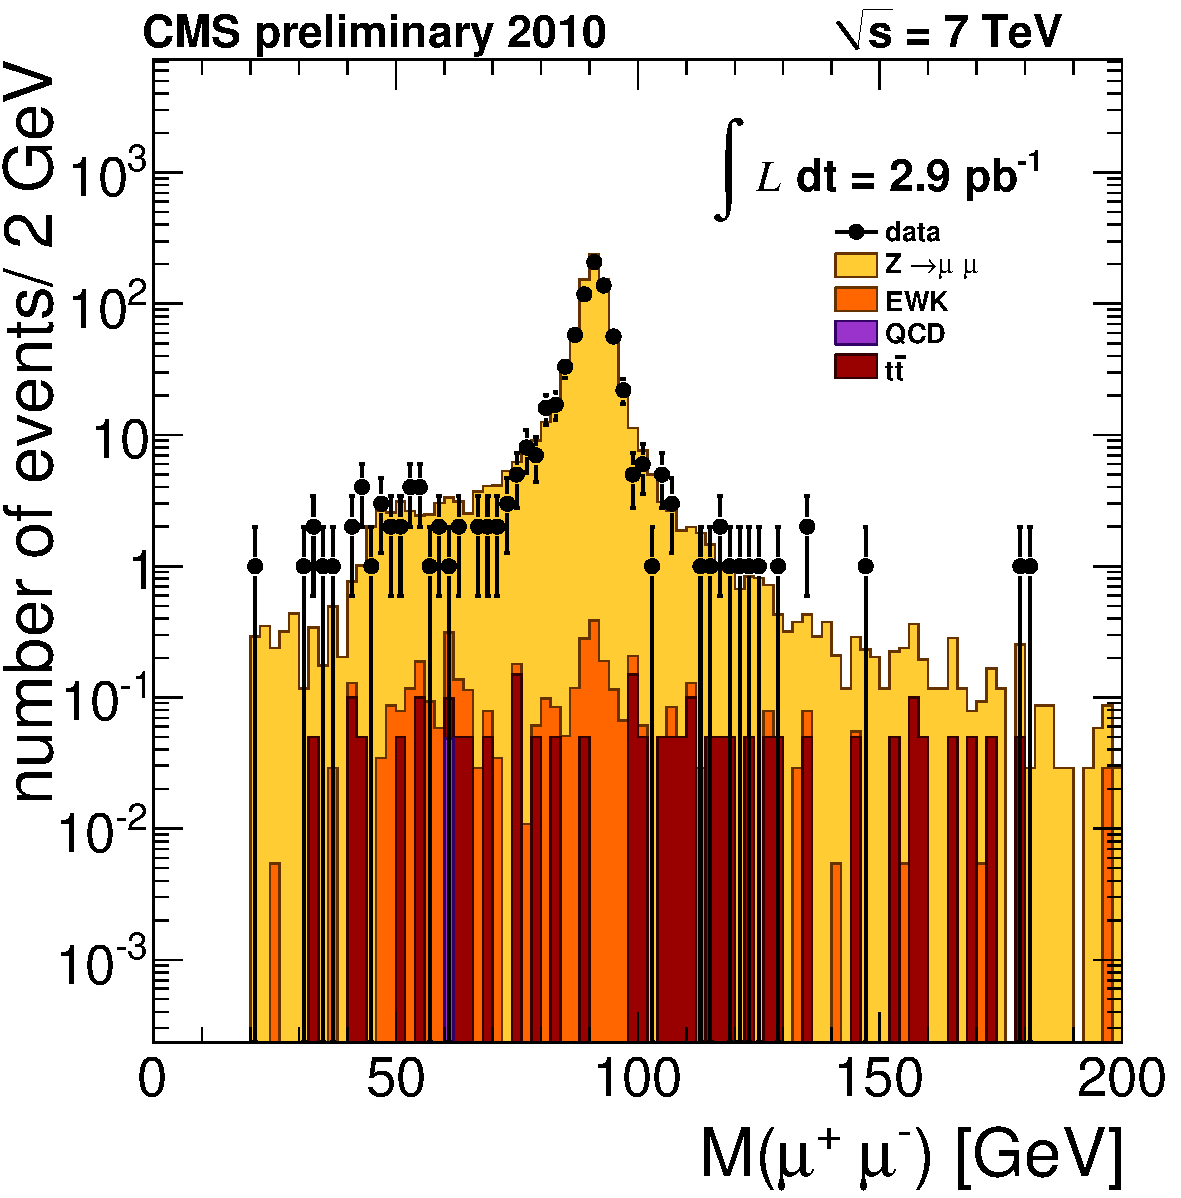
\includegraphics{FifthChapter/zmm_2hlt_2p9pb_log.pdf}
}
\caption{Invariant mass distribution of $\ZmumuTwoHlt$ candidates for
  data and MC signal and background events 
for  a luminosity of 2.9 pb$^{-1}$.}
  \label{fig:zmm_2hlt}
  \end{center}
\end{figure}

\begin{figure}[hbtp]
 \begin{center}
    \resizebox{0.55\textwidth}{!}{
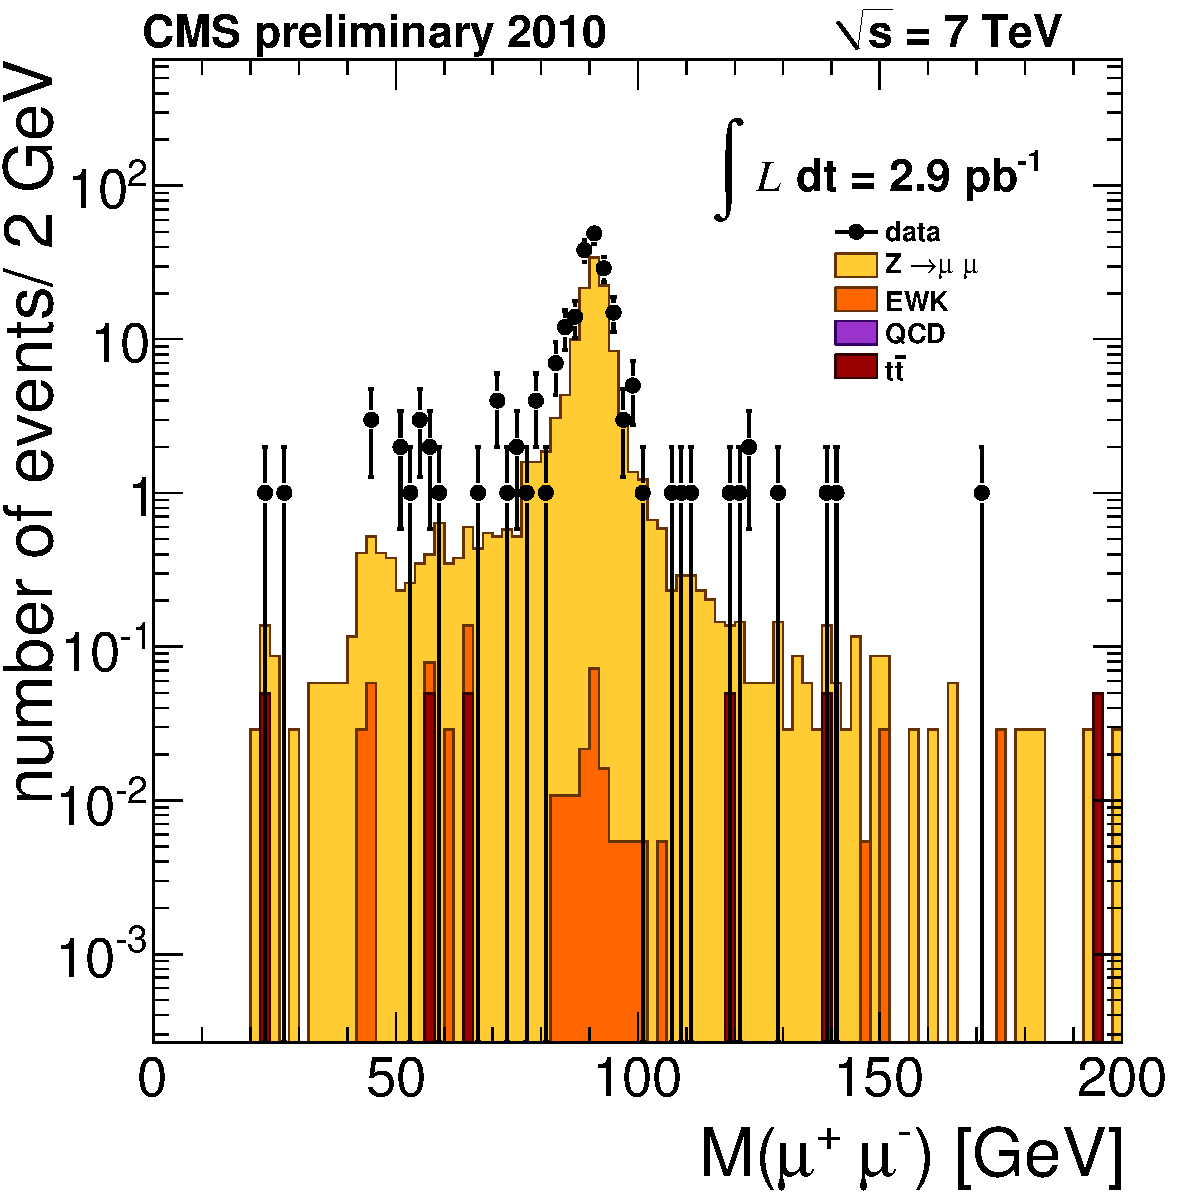
\includegraphics{FifthChapter/zmm_1hlt_2p9pb_log.pdf}
}
\caption{Invariant mass distribution of $\ZmumuOneHlt$ candidates for 
  data and MC signal and background events 
for  a luminosity of 2.9 pb$^{-1} $. The discrepancy one sees is due to the different $\effHlt$ in
data and simulation.}
  \label{fig:zmm_1hlt}
  \end{center}
\end{figure}
\begin{figure}[hbtp]
 \begin{center}
    \resizebox{0.55\textwidth}{!}{
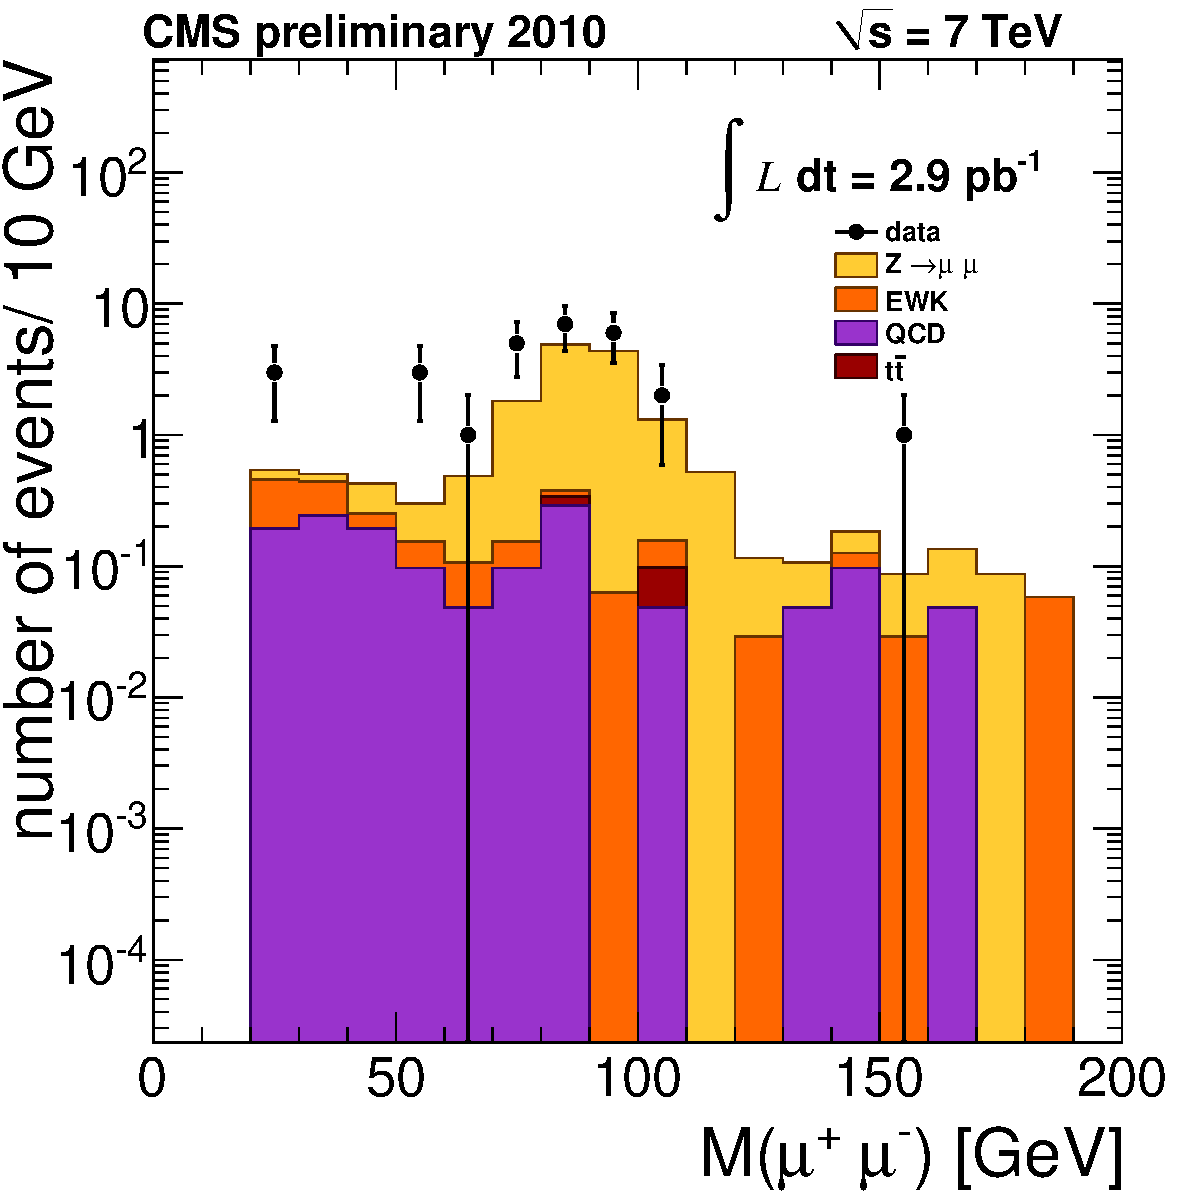
\includegraphics{FifthChapter/zms_log.pdf}
}
\caption{Invariant mass distribution of $\Zmus$ candidates for
  data and MC signal and background events 
for  a luminosity of 2.9 pb$^{-1}$.}
  \label{fig:zms}
  \end{center}
\end{figure}
\begin{figure}[hbtp]
 \begin{center}
    \resizebox{0.55\textwidth}{!}{
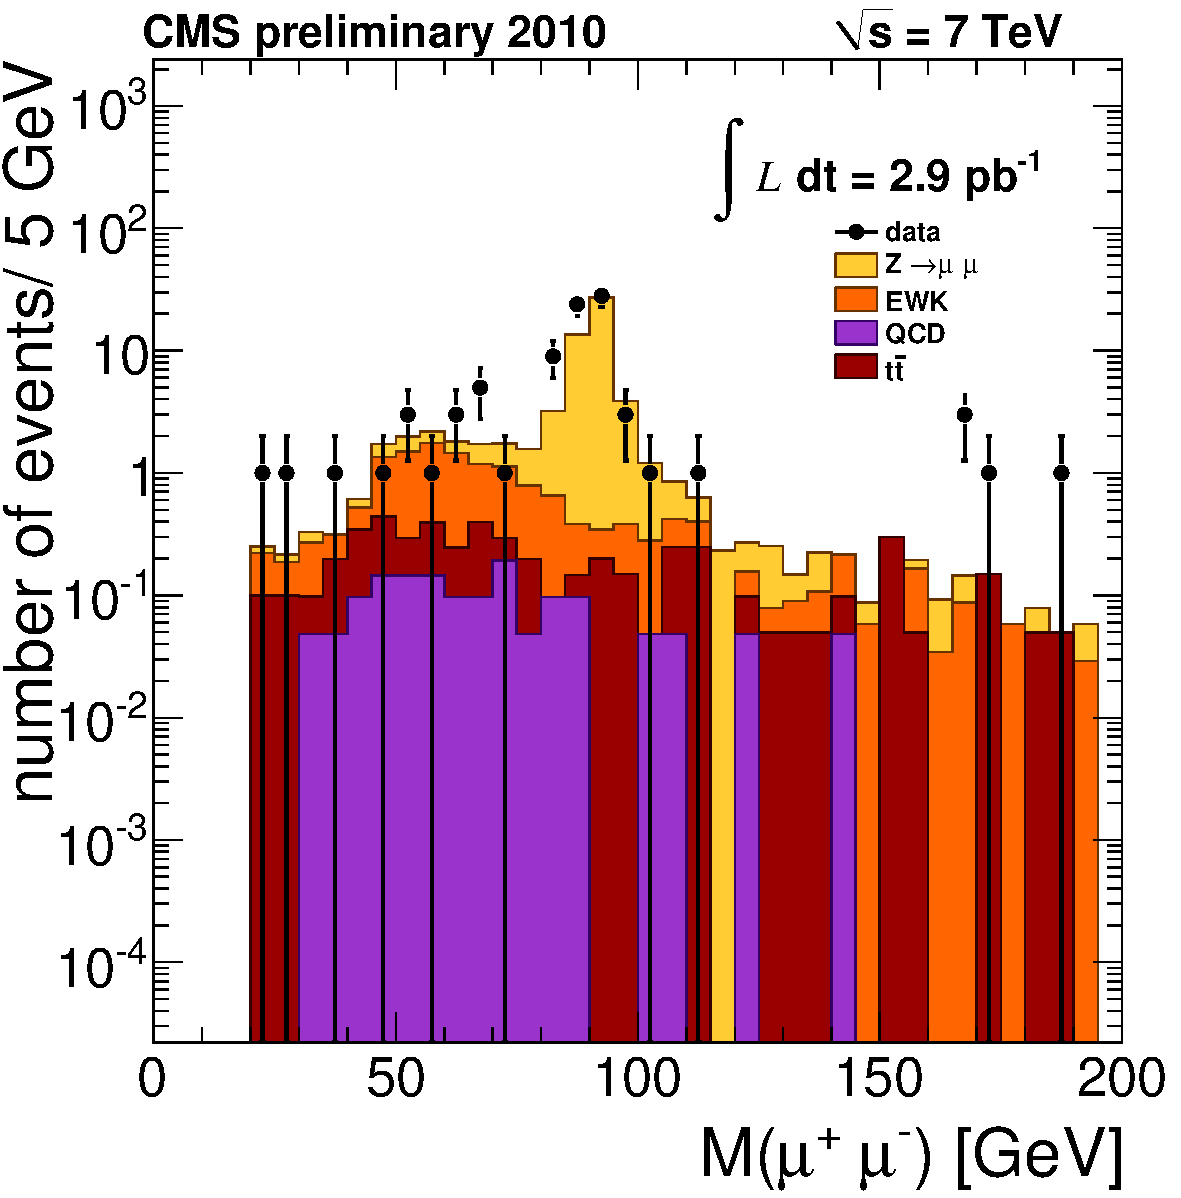
\includegraphics{FifthChapter/zmt_log.pdf}
}
\caption{Invariant mass distribution of $\Zmut$ candidates for
  data and MC signal and background events 
for  a luminosity of 2.9 pb$^{-1}$.}
  \label{fig:zmt}
  \end{center}
\end{figure}

\begin{figure}[hbtp]
 \begin{center}
    \resizebox{0.55\textwidth}{!}{
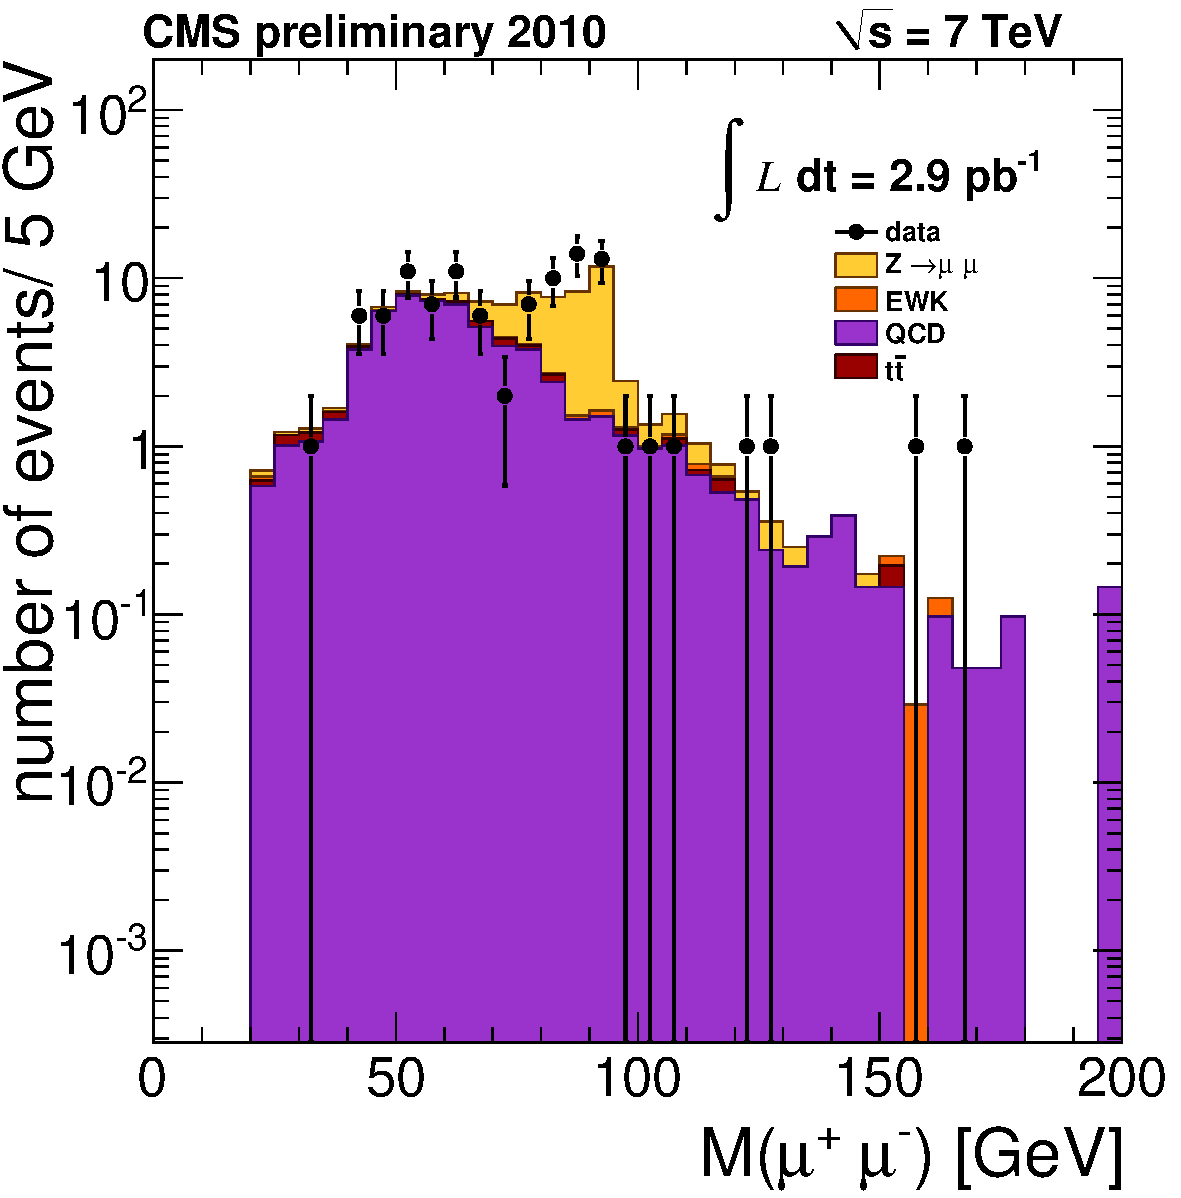
\includegraphics{FifthChapter/zNoIso_log.pdf}
}
\caption{Invariant mass distribution of $\ZmumuNonIso$ candidates for
  data and MC signal and background events 
for  a luminosity of 2.9 pb$^{-1} $.}
  \label{fig:zNoIso}
  \end{center}
\end{figure}

\begin{table}[htbp]
\vspace{0.5cm}
\begin{center}
\begin{tabular}{|l|c|c|c|c|}
\hline
 sample & $\Zmumu$ & $\Zmus$ & $\Zmut$ & $\ZmumuNonIso$ \\ 
\hline\hline
$  Z \rightarrow\mu^+\mu^-$ & $950 \pm 6$ & $12.5 \pm 0.6$ & $50.2 \pm 1.2$ & $33.3 \pm 1.0$ \\
\hline
$ W^\pm \rightarrow\mu^\pm \nu_{\mu}$ & $0.03 \pm 0.03$ & $0.23 \pm 0.08$  & $2.0 \pm 0.2$ & $0.55 \pm 0.12$ \\
\hline
$ t\bar{t}$ & $1.3 \pm 0.2 $ & $0.10 \pm 0.06$  & $1.5 \pm 0.3$ & $1.9 \pm 0.3$ \\
\hline
QCD & $0.05 \pm 0.05$  & $0.5 \pm 0.2$  & $0.7 \pm 0.2$ & $29.6 \pm 1.2$ \\
\hline
$Z \rightarrow\tau^+\tau^-$ & $0.52 \pm 0.12$ & $0.03\pm 0.03$ & $2.6 \pm 0.3$ & No events \\
\hline
$WZ$ & $0.72 \pm 0.06$ & $0.011 \pm 0.007$ & $0.10 \pm0.02$ & $0.06 \pm 0.02$ \\
\hline
$WW$ & $0.32 \pm 0.09$ & No events & $0.38 \pm 0.10$ & No events \\
\hline
$ZZ$ & $0.55 \pm 0.13$ & No events & $0.09 \pm 0.05$ &  $0.06 \pm 0.04$\\
\hline \hline
data & 913& 21& 75 & 66\\
\hline
\end{tabular}
\end{center}
\caption{Number of candidates expected (MC) and selected (data) in each category with an invariant mass
in the range [60-120] GeV$/c^2$ for 2.9 pb$^{-1}$ in data and MC. Here  $\Zmumu = \ZmumuOneHlt + \ZmumuTwoHlt$. 
For MC the separate contributions from signal and background processes are shown.}
\label{tab:2p9pb_selection}
\end{table}


\subsection{Fit results}
We have performed the fit on the 2.9 pb$^{-1}$ 7 TeV collision data.
Figures~\ref{fig:zmut_fit}-\ref{fig:zNoIso_fit} show the fit result 
superimposed to the histograms for the $\Zmus$, $\Zmut$, and $\ZmumuNonIso$ 
samples. Table~\ref{fitRes_2p9} reports the yield and efficiencies determined fro
m  the fit. They are compared to the results obtained by a fit performed using the 
the MC signal plus background only scaled to 2.9 pb$^{-1}$. In addition, the MC truth
values of the average efficiencies, obtained from a sample of \Zmm MC
signal events, are also reported in the Table. 
The resulting $\chi^2$ and correspondent $p$-value (i.e. the
probability of obtaining a value greater that the obtained one,
evaluated from the $\chi^2$ distribution) assures the goodness of the fit procedure.


From the fit results and the comparison with the MC-truth, one can see that all
the efficiencies found in data agree quite well with the expectation (even tough
slightly lower) with except of the trigger efficiency which is significant
lower in data, as we can  already see from the plots in Fig.
\ref{fig:zmm_1hlt} and \ref{fig:zmm_2hlt}, showing that the events in
the  $\ZmumuOneHlt$ are visible more than the expectation and the
contrary for the  $\ZmumuTwoHlt$ category.  This extra trigger 
inefficiency in data is however well know in the CMS community and
some more plots, reasons and discussion will be given in the following section \ref{TriggerZmumu}. 

Given the low statistics, the polynomial degree of the background shape
is truncated to the first order, and the $\Zmus$ histogram, wch
containes only about 20 entries, is supposed
to be background free (Table
\ref{tab:2p9pb_selection} shows that the background expected fraction  is about 10\%, not possible to subtract
with such a low number of entries). 

The correlation coefficients of the fit parameters is reported for completeness in
Table \ref{tab:fitMatrixCorrelations}. The first line of the matrix correlation
table reports the correlations between the $Z$ yield and the other fit
parameter. No correlations greater than 13\% are present.

An additional test is doing evaluating the poissonian likelihood ratio
variation from the minimum versus the yield value (after fixing all the efficiency term
parameter in the fit). This variation is compared to an ideal Gaussian
parabolic shape as a function of the $Z$ yield, where the $\sigma$ of the Gaussian is fixed to the
yield one standard deviation error around the best fit minimum.  So we
can safely consider a Gaussian approximation to evaluate the error of the fitted \Zmm
yield. The comparison is shown in Fig. \ref{fig:LPRversusParabola}.



\begin{figure}[hbtp]
\begin{center}
    \resizebox{0.7\textwidth}{!}{
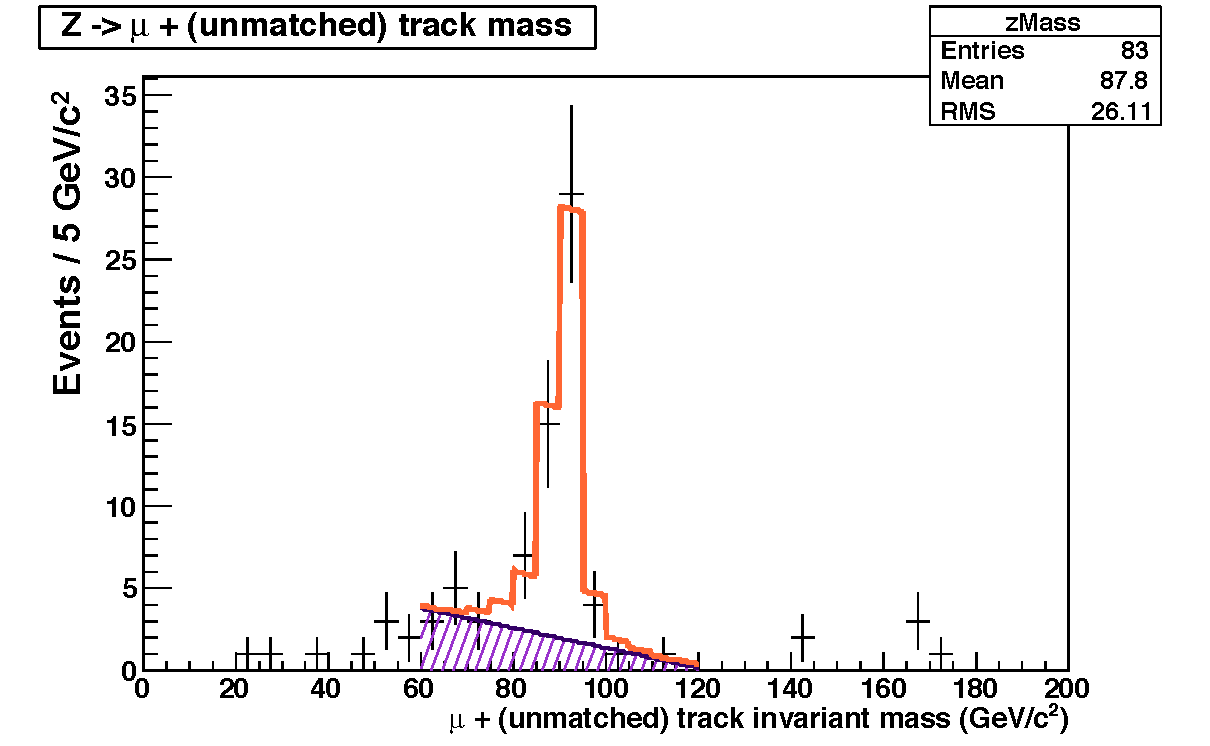
\includegraphics{FifthChapter/lin_ZMuTkFit_analysis_2p9.pdf}
}
\caption{Fit curve superimposed to the invariant mass histogram of 
$\Zmut$ candidates for $2.9$ pb$^{-1}$ of LHC 7 TeV collision data.}
  \label{fig:zmut_fit}
  \end{center}
\end{figure}

\begin{figure}[hbtp]
\begin{center}
    \resizebox{0.7\textwidth}{!}{
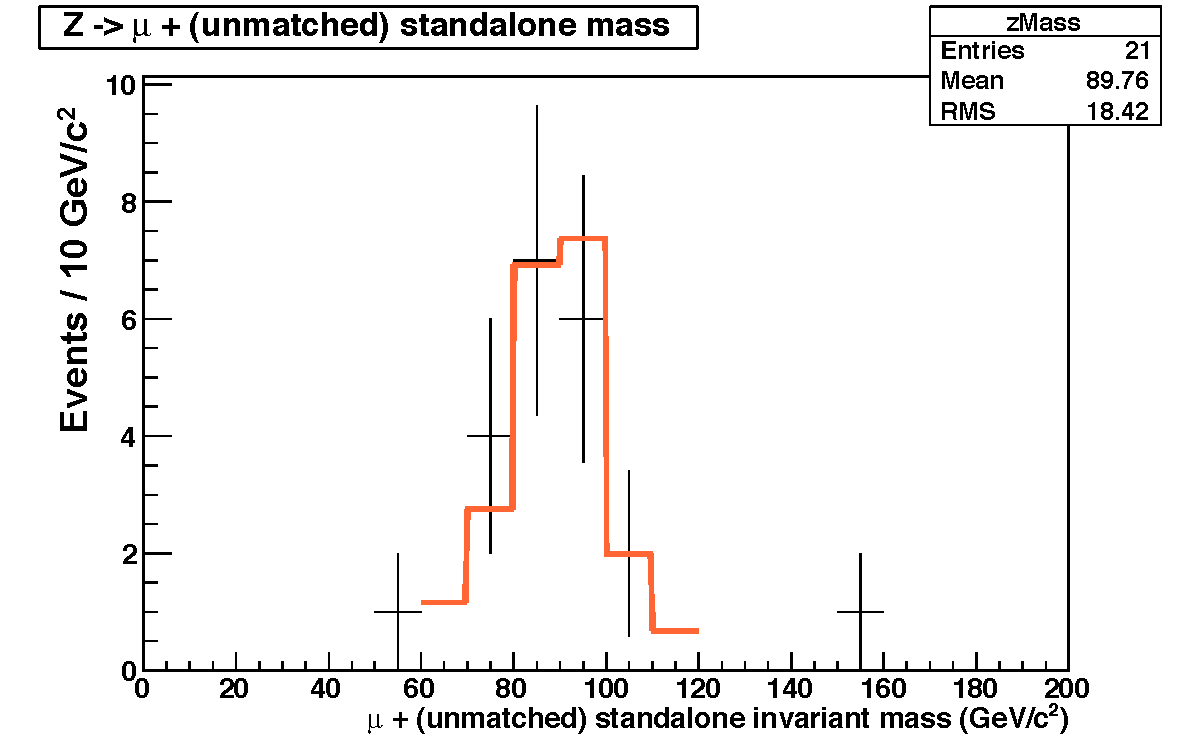
\includegraphics{FifthChapter/lin_ZMuSaFit_analysis_2p9.pdf}
}
\caption{Fit curve superimposed to the invariant mass histogram of 
$\Zmus$ candidates for a sample corresponding to an integrated luminosity of $2.9
$ pb$^{-1}$ of LHC 7 TeV collision data.}
  \label{fig:zmus_fit}
  \end{center}
\end{figure}

\begin{figure}[hbtp]
\begin{center}
    \resizebox{0.7\textwidth}{!}{
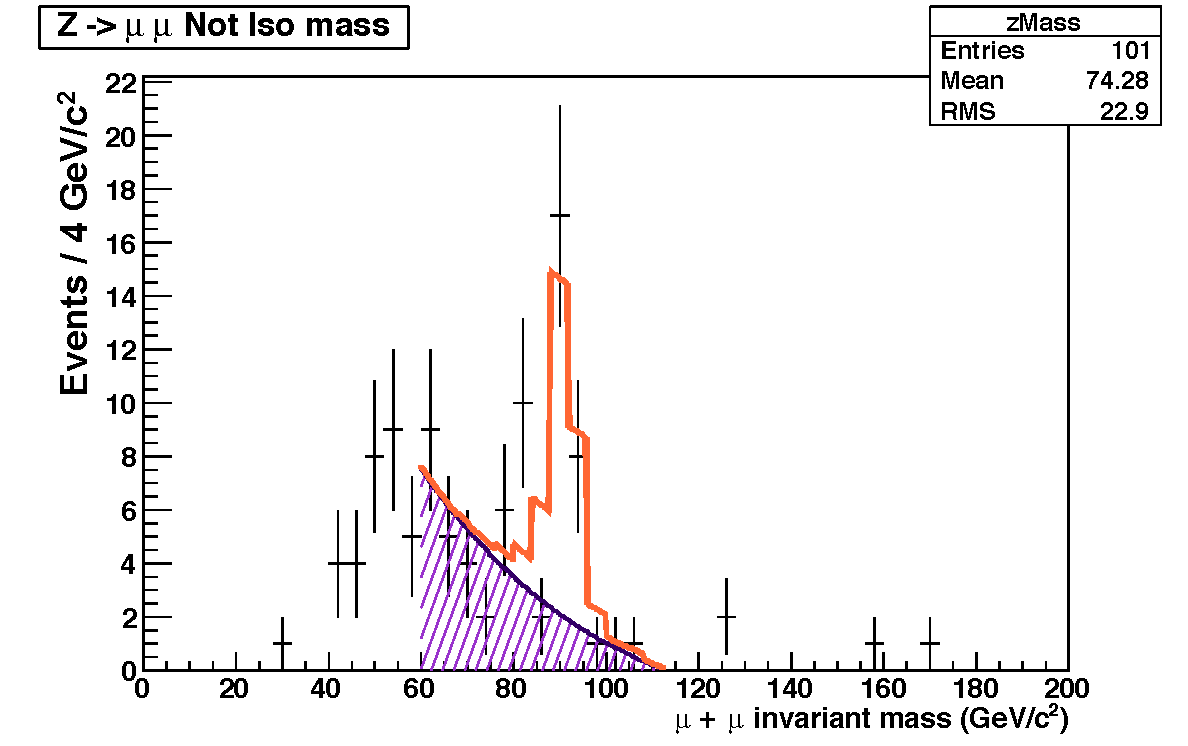
\includegraphics{FifthChapter/lin_ZMuMuNoIsoFit_analysis_2p9pb.pdf}
}
\caption{Fit curve superimposed to the invariant mass histogram of 
$\ZmumuNonIso$ candidates for a sample corresponding to an integrated luminosity
 of $2.9$ pb$^{-1}$ of LHC 7 TeV collision data.}
  \label{fig:zNoIso_fit}
  \end{center}
\end{figure}

\begin{table}[htbp]
\footnotesize
\begin{center}
\begin{tabular}{|c||c|c|c|c|c|c|c|c|c|c|c|}
\hline
Param.& Description& 1 &2&3&4&5&6&7&8&9&10\\ 
\hline\hline
\multirow{2}{*}{Yield} & \Zmm &
\multirow{2}{*}{1.000}&\multirow{2}{*}{-0.049}&\multirow{2}{*}{-0.126}&\multirow{2}{*}{-0.122}&\multirow{2}{*}{-0.081}&\multirow{2}{*}{-0.064}&\multirow{2}{*}{-0.055}&\multirow{2}{*}{0.036}&\multirow{2}{*}{0.052}&\multirow{2}{*}{-0.055}\\
 & yield& &&&&&&&&&\\
\hline
\multirow{2}{*}{$\effTrk$} & tracking & \multirow{2}{*}{-0.049}&\multirow{2}{*}{1.000}&\multirow{2}{*}{0.029}&\multirow{2}{*}{0.017}&\multirow{2}{*}{0.032}&\multirow{2}{*}{0.000}&\multirow{2}{*}{0.000}&\multirow{2}{*}{0.000}&\multirow{2}{*}{0.000}&\multirow{2}{*}{0.000}\\
& efficiency& &&&&&&&&&\\
\hline
\multirow{2}{*}{$\effSa$} & standalone& \multirow{2}{*}{-0.126}&\multirow{2}{*}{0.029}&\multirow{2}{*}{1.000}& \multirow{2}{*}{0.0024}&\multirow{2}{*}{0.045}&\multirow{2}{*}{0.000}&\multirow{2}{*}{0.177}&\multirow{2}{*}{-0.114}&\multirow{2}{*}{0.000}&\multirow{2}{*}{0.000}\\
& efficiency& &&&&&&&&&\\
\hline
\multirow{2}{*}{$\effIso$} & isolation & \multirow{2}{*}{-0.122}&\multirow{2}{*}{0.017}&\multirow{2}{*}{0.024}& \multirow{2}{*}{1.000}&\multirow{2}{*}{0.000}&\multirow{2}{*}{-0.270}&\multirow{2}{*}{0.000}&\multirow{2}{*}{0.000}&\multirow{2}{*}{-0.220}&\multirow{2}{*}{0.231}\\
& efficiency& &&&&&&&&&\\
\hline
\multirow{2}{*}{$\effHlt$} & trigger& \multirow{2}{*}{-0.081}&\multirow{2}{*}{0.032}&\multirow{2}{*}{0.045}& \multirow{2}{*}{0.000}&\multirow{2}{*}{1.000}&\multirow{2}{*}{0.000}&\multirow{2}{*}{0.000}&\multirow{2}{*}{0.000}&\multirow{2}{*}{0.000}&\multirow{2}{*}{0.000}\\
& efficiency& &&&&&&&&&\\
\hline
\multirow{2}{*}{$\alpha$} & background & \multirow{2}{*}{-0.064}&\multirow{2}{*}{0.000}&\multirow{2}{*}{0.000}& \multirow{2}{*}{0.270}&\multirow{2}{*}{0.000}&\multirow{2}{*}{1.000}&\multirow{2}{*}{0.000}&\multirow{2}{*}{0.000}&\multirow{2}{*}{-0.957}&\multirow{2}{*}{0.932}\\
& exponential slope   &&&&&&&&&&\\
\hline
\multirow{2}{*}{$A_0$} & $\Zmut$ bkg  polyn.& \multirow{2}{*}{-0.055}&\multirow{2}{*}{0.000}&\multirow{2}{*}{0.177}& \multirow{2}{*}{0.000}&\multirow{2}{*}{0.000}&\multirow{2}{*}{0.000}&\multirow{2}{*}{1.000}&\multirow{2}{*}{-0.978}&\multirow{2}{*}{0.000}&\multirow{2}{*}{0.000}\\
&1$^{st}$ degree term &&&&&&&&&&\\
\hline
\multirow{2}{*}{$A_1$} & $\Zmut$ bkg  polyn. &\multirow{2}{*}{0.036}&\multirow{2}{*}{0.000}&\multirow{2}{*}{-0.114}&
\multirow{2}{*}{0.000}&\multirow{2}{*}{0.000}&\multirow{2}{*}{0.000}&\multirow{2}{*}{-0.978}&\multirow{2}{*}{1.000}&\multirow{2}{*}{0.000}&\multirow{2}{*}{0.000}\\
&2$^{nd}$ degree term &&&&&&&&&&\\
\hline
\multirow{2}{*}{$B_0$} & $\ZmumuNonIso$ bkg  polyn. & \multirow{2}{*}{-0.052}&\multirow{2}{*}{0.000}&\multirow{2}{*}{0.000}& \multirow{2}{*}{-0.220}&\multirow{2}{*}{0.000}&\multirow{2}{*}{-0.957}&\multirow{2}{*}{0.000}&\multirow{2}{*}{0.000}&\multirow{2}{*}{1.000}&\multirow{2}{*}{-0.995}\\
&1$^{st}$ degree term &&&&&&&&&&\\
\hline
\multirow{2}{*}{$B_1$} & $\ZmumuNonIso$ bkg polyn.& \multirow{2}{*}{-0.055}&\multirow{2}{*}{0.000}&\multirow{2}{*}{0.000}& \multirow{2}{*}{0.231}&\multirow{2}{*}{0.000}&\multirow{2}{*}{0.932}&\multirow{2}{*}{0.000}&\multirow{2}{*}{0.000}&\multirow{2}{*}{-0.995}&\multirow{2}{*}{1.000}\\
&2$^{nd}$ degree term &&&&&&&&&&\\
\hline
\end{tabular}
\end{center}
\caption{Correlation coefficients of the fit parameters from the
  simultaneous fit minimization}
\label{tab:fitMatrixCorrelations}
\end{table}











\begin{table}[htbp]
\begin{center}
\begin{tabular}{|c||c||c|c|}
\hline
$\int L\mathrm{d}t = 2.9\mathrm{pb}^{-1}$ & fit results on data &
simulation (2.9$\mathrm{pb}^{-1}$) & MC-truth ef
ficiencies\\ 
\hline\hline
$\effHlt$ &0.883 $\pm$ 0.008  & 0.930 $\pm$0.007   & 0.9319 $\pm$ 0.0014 \\
\hline
$\effIso$ & 0.985 $\pm$ 0.004 & 0.990 $\pm$  0.004 & 0.9914 $\pm$ 0.0004 \\
\hline
$\effSa$ & 0.964  $\pm$ 0.004 & 0.971 $\pm$ 0.004 & 0.9724 $\pm$ 0.0006 \\
\hline
$\effTrk$ & 0.994 $\pm$0.005  & 0.994 $\pm$ 0.004  & 0.9927 $\pm$ 0.0007 \\
\hline
$\NZtomumu$ & 1050 $\pm$ 35   & 1107 $\pm$ 37      & \\
\hline
$\chi^2$/ndof & 1.074 & 1.034 & \\
\hline
$p-\mathrm{value}$& 0.373 & 0.402 & \\
\hline
\end{tabular}
\end{center}
\caption{Comparison between fit parameters results with the fit model described
  in this chapter performed in data with simulation signal and
  background scaled to the data luminosity. $\chi^2$/NDOF and
  $p$-value are also requested. MC-truth values of the average efficiencies are also shown for comparison.}
\label{fitRes_2p9}
\end{table}



%\begin{figure}[hbtp]
%\vspace{0.5cm}
% \begin{center}
 %  \resizebox{1.0\textwidth}{!}{
%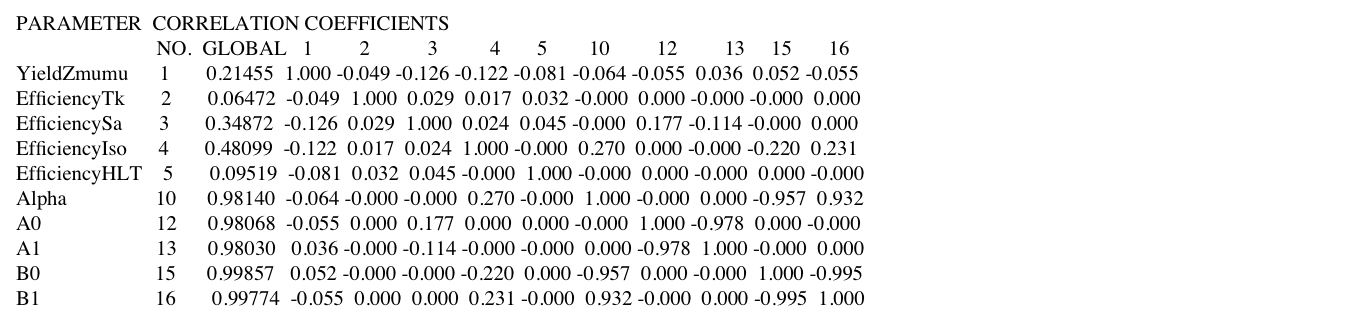
\includegraphics{FifthChapter/Fit2p9Correlations.pdf}
%}
%\caption{Correlation matrix from the simultaneous fit minimization}
 % \label{fig:fitMatrixCorrelations}
 % \end{center}
%end{figure}





\begin{figure}[hbtp]
\vspace{0.5cm}
 \begin{center}
    \resizebox{1.0\textwidth}{!}{
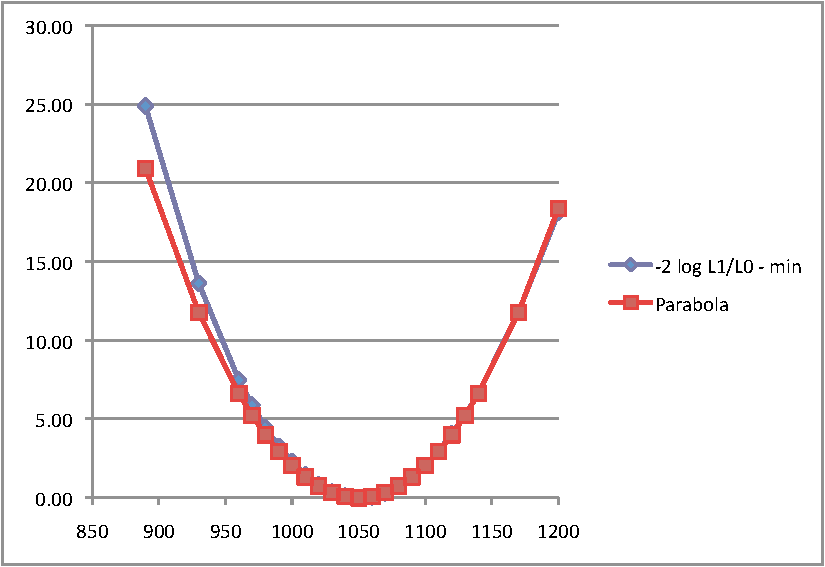
\includegraphics{FifthChapter/LPRversusParabola.pdf}
}
\caption{Poissonian likelihood ratio
variation from the minimum versus the yield value compared with a
Gaussian parabola.}
  \label{fig:LPRversusParabola}
  \end{center}
\end{figure}

\subsection{Kinematic acceptance}
\label{acceptance}
Once the \Zmm yield has been determined, we need to evaluate the kinematic acceptance
at generator level in order to determine the cross-section in an
enlarged kinematic region. 

The acceptance of the applied kinematic selection
can be evaluated with Monte Carlo, and is somewhat sensitive
to the generator adopted. 

Aiming to determine the cross section in the same mass region used in
the fit, but without any $p_T$ and $\eta$ cut the acceptance we need
to correct is:

\begin{equation}
\epsilon^{\mathrm{kin}} = \frac{N ( 60< m_Z<120,
  p_{T, \mu}>20,  |\eta_{\mu}|<2.1)}{N( 60<m_Z<120)},
\end{equation}
where the numerator of the formula is the number of events considering muon
after the final state radiation (because these are the muons we
detect), while in the denominator the mass of the dimuon system is
evaluated before the final state radiation. That is done in order to
compare the final cross-section number with a theoretical prediction
which includes also the final state radiation in the calculation.

Running on the MC \Zmm sample used for the analysis I found for the
geometric acceptance the value is:

\begin{equation}
\epsilon^{\mathrm{kin}} = 0.3977 \pm 0.0017.
\end{equation}


In order to use the Monte Carlo estimate, we need to 
verify that the acceptance estimated on generator particle
and on reconstructed muons is identical and not affected too much from 
resolution effects.  The good agreement has  been verified in data
with the statistics got so far and
the relative systematics quoted as 0.2\%. 





\subsection{Systematic Uncertianties}\label{subsec:systematics}
We can account for sources of systematics to  the \Zmm cross-section
measurement the followings:

\begin{itemize}

\item The first source of systematic uncertainty is the LHC machine luminosity estimate which
amount to 11\% \cite{CMSLumi} and will be quoted separately in the final number.

\item A second source is the theoretical uncertainty which affect the
acceptance, due to the uncertainties  on parton density function. On top of higher order QCD corrections, an  attempt has
been carried on to estimate the effect of Electroweak diagrams
not fully implemented in our baseline MC: final state radiation and
virtual and non-virtual corrections. A complete list of results can be
found in \cite{AN_2010_264}.

\item A subtle source of systematics due to the on-line data taking, hence
the L1 trigger, is the loss of muon events for trigger pre-firing, i.e. wrong assignment to the muon(s) bunch crossing
number. This
effect is due to wrong timing in the  DT, CSC and RPC system, and is
especially affecting the muon system overlap region ($0.9 < |\eta| <
1.2$) in which one should take care not only on the timing of the DT,
CSC or RPC only, both also on the synchronization of the three
subsystems. Anyway the correction to be applied for those timing
problem has been estimated for the current data to be at maximum
$1.0 \pm 0.5\%$ for the \Zmm channel. This estimate has been
obtained searching events in which a standalone-standalone pair of
muons, peaking at the $Z$ mass value is found: muon pre-firing 
indeed role out the tracker system from the muon measurements,
resuting in the impossibility to built a L3 muon online and a global
muon in the offline reconstruction.  We just remark that it is a global
scale factor to the cross-section (to be enhanced by 1\%, becuase we loss
these 1\% of events) and the 0.5\%
uncertainty is taken as systematic uncertainty.


\item The remaining sources of systematics are then the one introduced
with the fit procedure. 

We build the probability functions for the signal in a fully data
driven way. The same is not true for the
background shape, built as polynomial of first degree times
an exponential.  We tried to change the background from first to second
degree polynomial functions, then to fix to zero the slope of the exponential and then vary the binning.  The fit yield value is very stable.
So we took half the difference between the max and min fitted yield,
and we assigned it as systematic error. We estimate a 0.7\%
uncertainty due to this effect. 

The $\ZmumuTwoHlt$ and $\ZmumuOneHlt$ histograms are supposed
to be background free, but we know form MC that we have an irreducible
contamination of less than 0.5\% with the given selection. 
We added a flat background contribution to the two 
histograms and we saw that the fit yield output changes by an amount
of 0.3 $\times$  the backgorund over signal ratio. So we can quote as 0.2\% as a conservative
estimate of systematics error due to neglecting the background in the $\ZmumuTwoHlt$ and $\ZmumuOneHlt$ histograms.
  
Adding these two numbers in quadrature we can quote as a conservative
estimate for the fit systematics of 1\%.
\end{itemize}
Table \ref{tab:systematics} below reports all the contribution to the
systematics uncertaities to the the data driven \Zmm cross-section measurement.


\begin{table}[htbp]
\caption{Table of systematic uncertainties for the simultaneous fit \Zmm cross-section measurement. }
\label{tab:systematics}
\begin{center}
\begin{tabular}{ |  c | c |}
\hline
 Source & \%\\
\hline\hline
 Trigger firing & 0.5 \\
Muon momentum scale/resolution & 0.2 \\
Fit Background shape and subtraction & 1.0 \\
PDF uncertainty in acceptance & 1.2 \\
Other theoretical uncertainties & 1.6 \\   
\hline
TOTAL(without luminosity uncertainty) & 2.3 \\
\hline
Luminosity & 11.0 \\
\hline
\end{tabular}
\end{center}
\end{table}

\subsection{cross-section determination}

At this point all the ingredients to finally evaluate the \Zmm cross
section with the first 2.9 pb$^{-1}$ of 7 TeV collision data are available.

We start from the well known formula for the extraction of the
cross-section already introduced in the Equation \ref{eq:x-section}


As can be seen in Tab \ref{tab:2p9pb_selection} the expected
contamination of irreducible background, $f_{bkg}$,  in the
$\ZmumuTwoHlt$ and $\ZmumuOneHlt$  categories 
is $f_{bkg}=0.37\% $ (3.5 $\pm$ 0.3 events on a total of 950 expected
signal events). \footnote{From the Table \ref{tab:2p9pb_selection}
  also one can see that the QCD contribution to the background is very
  little w.r.t. other EWK channels and
$t\bar{t}$. So we don't need to care for any possble increase of the
QCD contribution w.r.t. to simulation where QCD (especially $b\bar{b}$) decay and
punch-troughts in the muon system are not correctly simulated.  
This scale factor to apply to the QCD background has been anyway
estimated to be not greater than 1.5. As we subtract the background in
the other loose categories where the QCD is the main source of background,  we
don't need to consider this additional increment also for these
histograms.} 

The simultaneous fit strategy gives directly the Yield corrected by
the efficiencies to select the \Zmm candidates, so we  can evaluate the cross-section
as:

\begin{equation}
\sigma = \frac{Y (1 - f_{bkg})}{ A  \int \mathcal{L} dt }
\end{equation}

A 1\% correction due to the loss of muon events due to trigger
pre-firing in the first era of CMS data taking is also applied (as
explained in Section \ref{subsec:systematics}).
The following cross-sections for $Z$ production is then measured:

\begin{equation}
\footnotesize
\bf{\sigma (pp \rightarrow  ZX) \times BF ( Z \rightarrow \mu^+ \mu^-) = 0.924 � 0.031 (stat.) � 0.022 (syst.) � 0.101 (lumi.) nb},
\end{equation}

The reported $Z$ cross-sections is limited to the invariant mass range
60 < m$_{\mu^+ \mu^-}$ < 120 GeV/c$^2$, and
is corrected for the kinematic acceptance. The NNLO prediction for Z
production is 0.97 $\pm$ 0.04 nb, so we find very good agreement with the
Standard Model prediction.



\subsection{correction factors  for \Wmn analysis}
The \Wmn selection requires the presence of an high $p_T$ muon
accompanied by a significant amount of missing transerve energy in the
event. 

For the first \Wmn data driven measurement at CMS one needs to get the
correction factor DATA/MonteCarlo ($\rho_{eff}$) for the efficiencies
to reconstruct, trigger and identify a muon. That is done to correct
the efficiencies taken directly from the simulation in a way similar
to the one used in the first era of the \Zmm analysis, described in
Section \ref{sec:MCdrivenAnalysis} . 
The correction value for the \Wmn has been
obtained by mean of the simultaneous fit to the \Zmm sample described
in the note comparing the results obtained in data and simulation.  

The muon selection in the \Wmn
analysis is equivalent to the one used for the \Zmm except for two additional
requirements on the global muon track: the $\chi2$ of the fit to be
less than 10 and the requirement for the global muon to be also
a tracker muon. We will denote as $\epsilon_{sel}$ the efficiency for
the two additional cuts.  

With the \Zmm selected events we can  measured  $\epsilon_{sel}$ as a ratio of
di-muons from global-global pairs in the mass range with and without those cuts applied to
both muons (having applied fisrt all the other cuts).


The measurements of $\effHlt$, $\effIso$,
$\effTrk$, $\effSa$ on data and simulation has been already shown in
table \ref{fitRes_2p9}. Now we show the resulting correction factors and
the numerical values of $\epsilon_{sel}$. The total correction factor
$\rho_{eff}$ is the product of
all the corrections. A summary of the results is given in Table
\ref{tab:corrW}. 

\begin{table}[htbp]
\vspace{0.5cm}
\begin{center}
\begin{tabular}{|c||c||c|c|}
\hline
Efficiency & Data & Simulation &  Data/Simulation($\rho_{eff}$)\\ 
\hline\hline
$\effHlt$ &0.883 $\pm$ 0.008  & 0.9319 $\pm$ 0.0014  & 0.947 $\pm$ 0.009\\
\hline
$\effIso$ & 0.985 $\pm$ 0.004  & 0.9914 $\pm$ 0.0004  & 0.994 $\pm$  0.004\\
\hline
$\effSa$ & 0.964  $\pm$ 0.004 & 0.9724 $\pm$ 0.0006 & 0.992 $\pm$ 0.005 \\
\hline
$\effTrk$ & 0.994 $\pm$0.005  & 0.9927 $\pm$ 0.0007 & 0.998 $\pm$ 0.003   \\
\hline
$\epsilon_{sel}$ & 0.997 $\pm$0.003  & 0.9967 $\pm$ 0.0005 & 1.0 $\pm$ 0.003   \\
\hline\hline
Net($W$) & 0.828 $\pm$ 0.011  & 0.8874 $\pm$ 0.0013  &  \bf{0.933 $\pm$ 0.012}\\
\hline
\end{tabular}
\end{center}
\caption{Final efficiency factors used in the \Wmn analysis. There
  were obtained applying the simultaneous fit  technique on a clean  \Zmm sample.}
\label{tab:corrW}
\end{table}



As can be seen in the table, most of the correction numeric values
are very close to unity. Only the trigger efficiency is about 5\%
lower in data than in simulation, a fact that has been confirmed many
times in CMS and will be discussed in the next Section.


\begin{table}[htbp]
\vspace{0.5cm}
\begin{center}
\begin{tabular}{|c|c|}
\hline
Subset &  Data/Simulation(Net $\rho_{eff}$)\\ 
\hline\hline
positive muons &   0.935 $\pm$ 0.018\\
negative muons &   0.931 $\pm$ 0.019\\
\hline
barrel ($|\eta| <0.9$) &   0.955 $\pm$ 0.024\\
transition (0.9 < $|\eta| <1.2$) &   0.89 $\pm$ 0.04\\
endcap (1.2 < $|\eta| <2.1$) &   0.92 $\pm$ 0.03\\
\hline
\end{tabular}
\end{center}
\caption{Correction factors for subsets of muons}
\label{tab:corrMupMumEB}
\end{table}
Additional studies performed with the \Zmm selection and analysis
strategy essential for the \Wmn analysis one are the following:
\begin{itemize}
\item We evaluated the correction factors for positive and negative muons separately, as shown
in Table \ref{tab:corrMupMumEB}. The difference amounts to 0.4\% and is
compatible with zero. Hence the same correction can be applied for
the $W^{+} \rightarrow \mu^{+} \nu$ and $W^{-} \rightarrow \mu^{-}
\nu$  and in the ratio $W^{+} / W^{-}$.
\item The table also lists the correction values for the barrel, endcap and transition regions of
the muon system. The correction factors are fairly uniform with
perhaps a somewhat lower value in the transition, or overlap region
between the DTs and the CSCs.
\item Another important result found is the global correlation between the
product of the efficiencies for the muon selection and the \Zmm
yield. This number is used for the error propagation in the  W
over $Z$ ratio, which is one of the most important EWK measurement ........
This value has been obtained from the simultaneous  fit described
above reparametrizing one of the efficiency as $\epsilon_{tot} = \effHlt
 \effTrk \effSa \effIso $, and introducing this parameter in the fit
 minimization. The total correlation found is 
\begin{equation}
correlation(Yield, \epsilon_{tot}) = -0.236
\end{equation}
 
\end{itemize}

\newpage 

\subsection{Trigger efficiency estimate using \Zmm}\label{TriggerZmumu}

Dimuon resonance such as $J/\Psi$, $\Upsilon(1s)$, $Z$ are used to study the detector
reconstruction, isolation and trigger efficiencies using the so called
``Tag and Probe'' method. This method, which has been successfully
used in some form or another by past and present experiments, relies upon \Zmm decays to provide
 an unbiased, high-purity, muon sample with which to measure the
 efficiency of a particular selection cut, including the trigger. With
 the intention to study the trigger efficiency, a single muon trigger
 sample is used, from which a subset of di-muon events are
 selected. One of the muons, the ``tag'', is required to pass
 stringent muon identification criteria in order to have as low
 background as possible, while the other muon,
the ``probe'', is only required to pass a set of identification criteria depending on the efficiency under study. The
invariant mass of the tag and probe muon candidates is required
to be within a window around $m_Z$ . The tight criteria imposed on the tag coupled to the invariant mass requirement is sufficient to ensure high muon purity. 

This method has been applied to study the muon trigger efficiency,
to study the single muon trigger selection path named
{\tt{HLT\_Mu9}}. Both tag and prob muons  are required to pass
stringent identification and isolation cuts (see Section
\ref{sec:ICHEPSelection} ), in order to provide the efficiency to be
used for the \Wmn analysis. Hence the probe muon is required to pass
these tight identification and isolation cuts and the trigger firing
is investigated.

Applying this method we find for the average efficiency for $p_T>20 \:
GeV/c$ and $|\eta|<2.1$   in the first 2.9 $pb^{-1}$ of collision data
the value reported in Table \ref{tab:triggerZmm} and in the plots
of Fig. \ref{fig:triggerZmmEta} and \ref{fig:triggerZmmPt}. For comparison we
report also the efficiency we expect from the simulation, using the MC \Zmm simulated sample used in the note.
As already remarked the correction we found to be applied to pass from
simulated MC to data efficiency is of the order of 95\%, to be
precise $0.947 \pm 0.008$ for these tight selected
muons. 

The CMS community is investigating the reason of this ~5\% of
extra inefficiency in data. As can be seen by the numbers and plots it
is clear that the region much affected by thus trigger lost is the barrel-endcap
overlap region ($0.9 < |\eta| <2.1$), due to syncronization problem
between DT, CSC and RPC detectors. 
It has been found that all these subsystem need to better calibrate their timing
constants. That calibration can be done when more collision data will be available
and so it is expected that the L1 trigger efficiency will increase in
the near future.

In addition a second loss of efficiency has been found to be introduced in the L2 and L3 step,
expecially in the endcaps, due to a probability some per cent higher
than expected to assign a wrong charge to the muon in the L2-L3
steps.  For that reason new L3 algorithms will be
soon deployed on-line.



\begin{table}[htbp]
\footnotesize
\caption{Table of muon single muon trigger efficiency versus $\eta$
  obtained in data using the tag an prob method on  \Zmm selected event. }
\label{tab:triggerZmm}
\begin{center}
\begin{tabular}{ |  c | c | c| c| c|}
\hline
  & overall & barrel & transition region
  & endcaps \\
& (|$eta$|<2.1)&($|\eta| <0.9$)& (0.9< $\eta$<1.2) & ($1.2 < |\eta| < 2.1$)\\
\hline
\Zmm MC  & 0.9333 $\pm$ 0.0010 & 0.9607 $\pm$ 0.0012  & 0.871 $\pm$
0.003&  0.920 $\pm$ 0.002\\
\hline\hline
data (2.9 pb$^{-1}$) & 0.884 $\pm$ 0.007 & 0.934 $\pm$ 0.009& 0.75 $\pm$ 0.03& 0.871 $\pm$ 0.014\\
\hline
scale factor (data/MC) & 0.947 $\pm$ 0.008&  0.972 $\pm$ 0.010 & 0.86 $\pm$ 0.04& 0.947 $\pm$ 0.017\\
\hline
\end{tabular}
\end{center}
\end{table}



\begin{figure}[hbtp]
\vspace{0.5cm}
 \begin{center}
    \resizebox{0.8\textwidth}{!}{
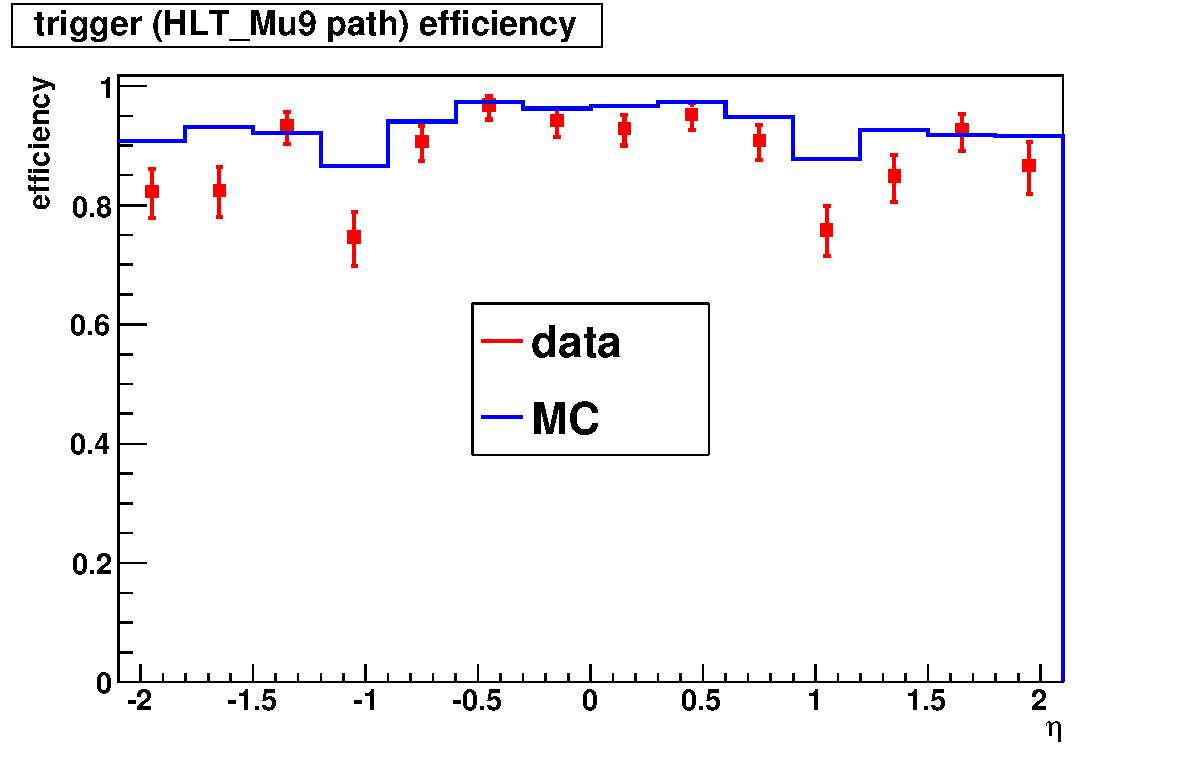
\includegraphics{FifthChapter/HLTMu9_eta_2p9pb.pdf}
}
\caption{Muon single muon trigger efficiency versus muon $\eta$,
  obtained using tag and prob method on \Zmm selected events on $2.9$ pb$^{-1}$ of LHC 7 TeV collision data.}
  \label{fig:triggerZmmEta}
  \end{center}
\end{figure}


\begin{figure}[h]
\vspace{0.5cm}
 \begin{center}
    \resizebox{0.8\textwidth}{!}{
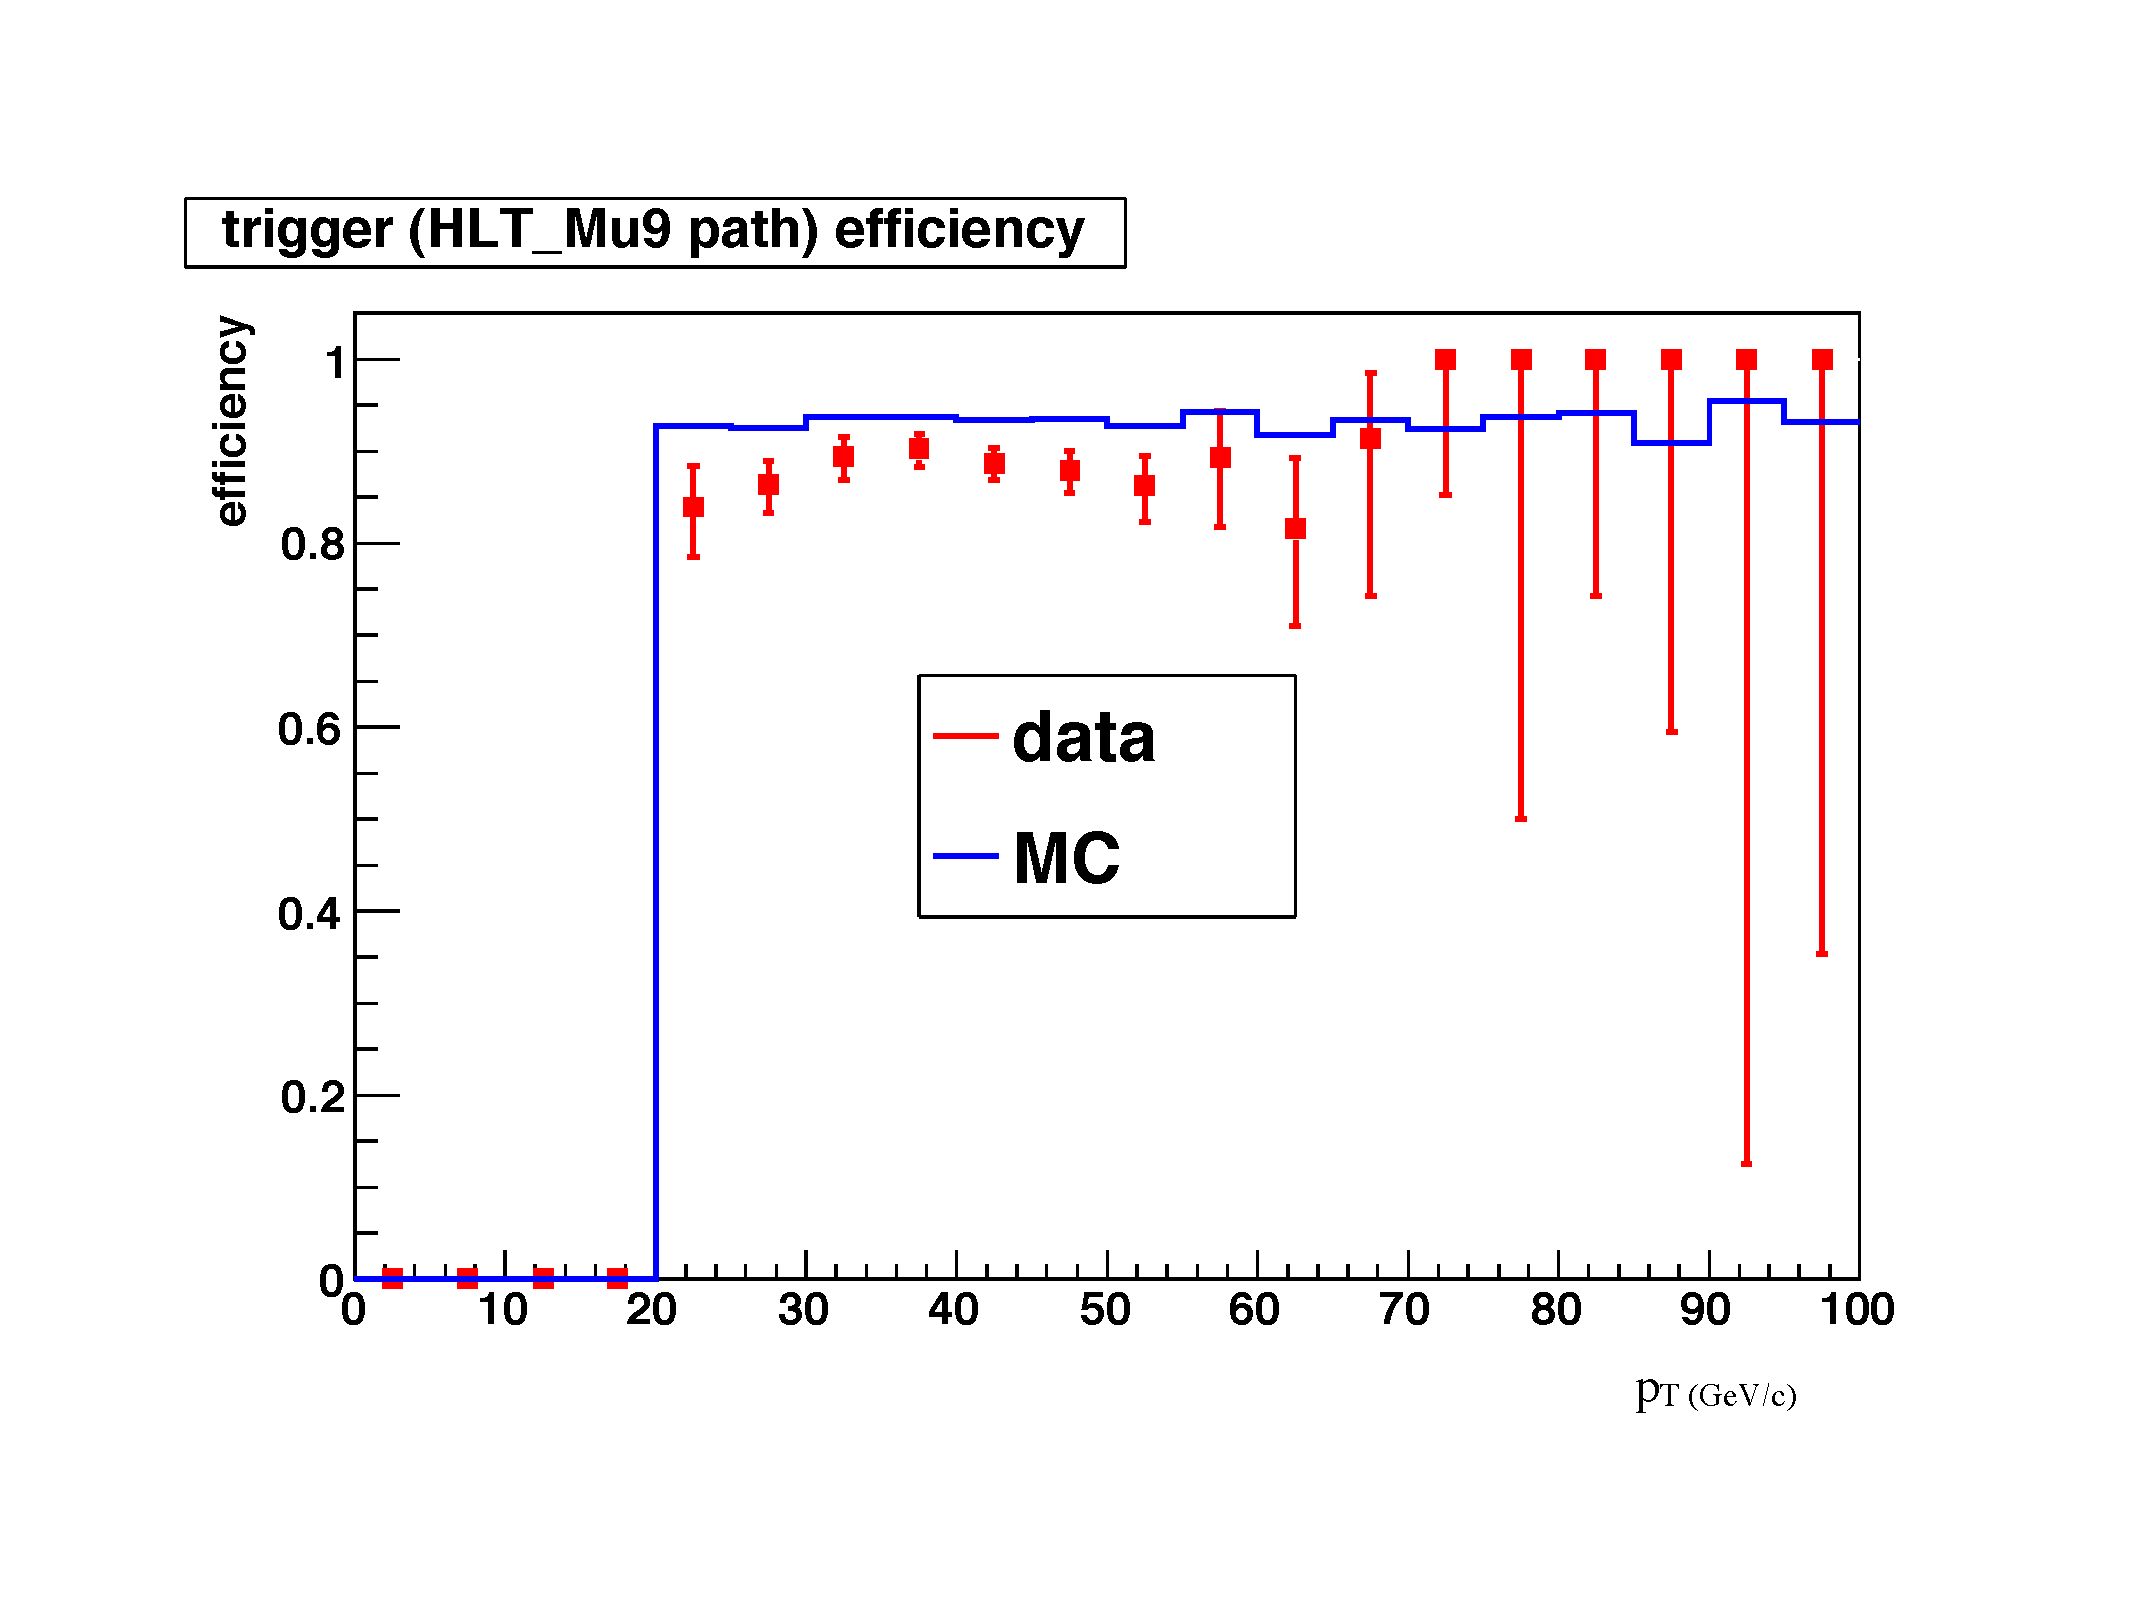
\includegraphics{FifthChapter/HLTMu9_pt_2p9pb.pdf}
}
\caption{Muon single muon trigger efficiency versus muon $p_T$ obtained using tag and
  prob method on \Zmm selected events on $2.9$ pb$^{-1}$ of LHC 7 TeV collision data.}
  \label{fig:triggerZmmPt}
  \end{center}
\end{figure}

\section{EWK results.....}

\subsection{Additional categories to check the background}
samecharge, 1 and 2 not iso ?????????? metterlo?????

\newpage

\section{Luminosity measurement using $W$ and $Z$}\label{sec:LumiFromZ}
The machine luminosity monitor and measurement is one of the most
important thing to assess in the first years of data taking of a new
accelerator and through-tout its whole life.

The integrated luminosity in CMS is based on signals from the Forward
Hadronic Calorimeter. Two methods for extracting a
real-time relative instantaneous luminosity are used. The ``zero
counting,'' method in which the average fraction of empty towers is
used to infer the mean number of interactions per bunch crossing. The
second method exploits the linear relationship between the average
transverse energy per tower and the luminosity. The choice of the
online algorithm chosen to report the luminosity summary might get
adjusted based on the data integrity/reliability namely the
statistical uncertainty or systematics uncertainty due to the Forward
Calorimeter or the background sensitivity. The different algorithm
agree to within 5\% so far. The final
normalization of the luminosity is based on Van der Meer scans, which determine the size of
the colliding beams and thus the luminosity with minimal reliance on simulation
 This techique was first pioneered by Van Der Meer at the ISR. See reference \cite{PerugiaLumi},
article to which I contributed, for a
review of the luminosity measurement issue at LHC, and \cite{CMSLumi}
for a details on the CMS measurement systematic uncertainties.

The resulting measurement is the most reliable one and the
recommended to be used for data analysis and is stored run by run ( to be
more precise lumisection by
lumisections, where the lumisections is the smallest part of a CMS
run lasting 23 s) in the CMS Condition Database and is accessible by the
whole CMS community.  

As already said the current precision of this method, resulting in a
systematics for all cross-section measurement is 11\% . The
uncertainty associated to this measurement is supposed to lower in
with the passing of the time, when all the LCH fill beam information
will be calibrated and measured always better, but is eventually
limited by the uncertainty  on the knowledge of all the QCD processes
contributing to the very forward physics. 

Several offline method have been used in the first era of the LHC:
above all the primary vertexes counting. The method counts the primary
vertices falling in each lumisections and knowing the expectation for
the theory manage to obtain a luminosity value for the
lumisections. As the on-line HF method also the vertex counting is
dominated finally by the QCD physics uncertainties.


With high integrated luminosity  we can exploit EWK channels, once the
Standard Model cross-section value will be definitely confirmed, to
use them as luminosity monitor and
eventually to measure the luminosity with low systematics. Muon
decays are for sure more feasible
for such a use, because in general CMS reaches better muon
reconstruction and identification than electrons. 
As already seen in the previous Section
already with about 3 $\mathrm{pb}^{-1}$ we have a measurement of the \Zmm cross
section in which the systematical error is comparable with the
statistical error, and it is neglecteble for the \Wmn channel, with
has about ten times graeter cross-section.

Already in the future year of the machine, when the instantaneous
luminosity will reach the value of $L = 10^{33} \mathrm{s}^{-1} \mathrm{cm}^{-2}$ we
will collect in less then 10 hours (hence a CMS run) an integrated
luminosity of the order of the pb$^{-1}$, and when the luminosity will
reach the design value of $L = 10^{34} \mathrm{s}^{-1} \mathrm{cm}^{-2}$  $W$ and Z
bosons decaying into muons will be produced with the rate of 10 and 1
Hz respectively.

Given that,  we found very useful to develop a tool, inserted in the offline DQM  framework,
that counts the number of selected \Wmn and \Zmm events and publishes
them on a web page.

The software program is run centrally with the complete DQM offline chain
producing the histogram containing  the \Zmm mass and \Wmn transverse mass
distribution. A subsequent script developed also by myself access the web
repository where this histograms are saved, counts the entries and
applies the data
driven method discribed in the previous Section and determine
the integrated luminosity (assuming that the Standard Model cross-section).

This tool has been put in place already with the first runs and shows
to agree well with the on-line measurements. We wait a larger instantaneous
luminosity to better exploit its utility with the resulting small uncertainties.

A snapshot of the \Wmn and \Zmm counting web page is shown in Figure~\ref{fig:Zcounting}

 \begin{figure}[hbtp]
\vspace{0.5cm}
 \begin{center}
    \resizebox{0.8\textwidth}{!}{
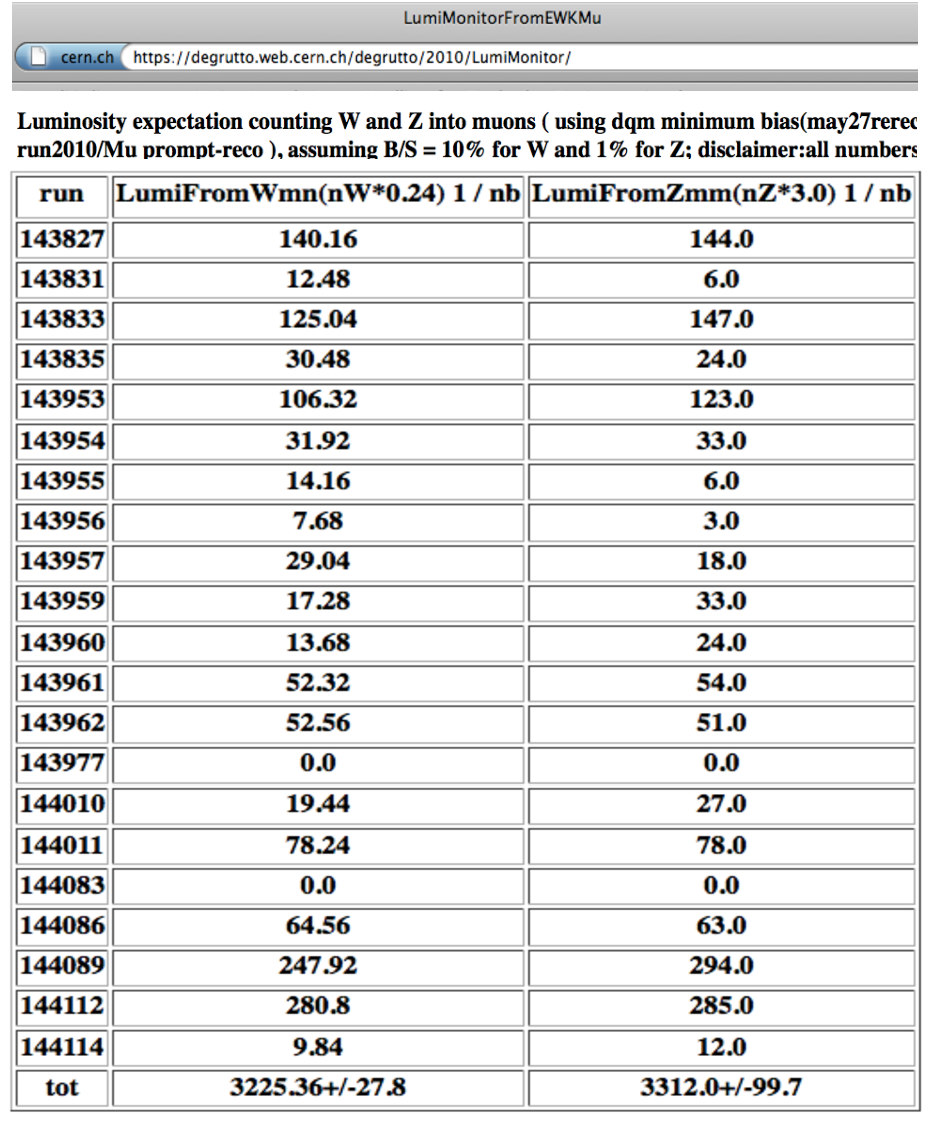
\includegraphics{FifthChapter/ZmmLumiMonitor_v2.pdf}
}
\caption{Snapshot of the web page produced with the offline luminosity
  measurement tool using $W$ and $Z$ bosons decaying into muons. The numbers
  are in nb$^{-1}$.}
  \label{fig:Zcounting}
  \end{center}
\end{figure}


%\bibliographystyle{unsrt}
\addcontentsline{toc}{chapter}{References}
\begin{thebibliography}{99}
\bibitem{EWKTheory1} S. L. Glashow, Nucl. Phys. 22, 579 (1961).
 \bibitem{EWKTheory2} S. Weinberg, Phys. Rev. Lett. 19, 1264 (1967).
January 2, 2009 14:52 WSPC - Proceedings 
\bibitem{EWKTheory3} A. Salam In Elementary Particle Theory, ed. N. Svartholm (Almquist and
Wiksells, Stockholm 1969), 367-377.
\bibitem{Langacker:2009my} P.~Langacker, ``Introduction to the Standard Model and Electroweak Physics,'' arXiv:0901.0241 [hep-ph].
\bibitem{Goldstone} J. Goldstone, A. Salam and S. Weinberg, Phys. Rev. 127, 965 (1962).
\bibitem{Gargamelle} F J Hasert et al. 1973a Phys. Lett. 46B 121.
\bibitem{UA1} G. Arnison et al., Phys. Lett. B166, p. 484 (1986).
\bibitem{UA2} R. Ansari et al., Phys. Lett. B186, p. 440 (1987).
\bibitem{Altarelli} New Physics and the LHC. Guido Altarelli, (Rome III U. \& INFN, Rome3 \& CERN) . RM3-TH-08-9, CERN-PH-TH-2008-085, May 2008. 35pp. 
\bibitem{LEPHiggsLimit} The LEP Electroweak Working Group, http://lepewwg.web.cern.ch/LEPEWWG/
\bibitem{HiggsTeV} T. Aaltonen et al. (CDF and D0 Collaborations), Phys. Rev. Lett. 104, 061802 (2010).
\bibitem{ExtraDim} For a review and a list of references, see, for example, J. Hewett and M.
Spiropulu, Ann.Rev.Nucl.Part.Sci. 52, 397 (2002), hep-ph/0205196.
\bibitem{TOPPAS} CMS Collaboration, ``Selection of Top-Like Events in the Dilepton and Lepton-plus-Jets Channels in Early 7 TeV Data'', CMS-PAS-TOP-10-004. 
\bibitem{SUSYPAS} CMS Collaboration, ``Performance of Methods for Data-Driven Background Estimation in SUSY Searches'', CMS-PAS-SUS-10-001. 
\bibitem{ATLASHIGGS} ATLAS Collaboration, Expected performance of the ATLAS experiment: detector, trigger, physics, CERN Report, CERN-OPEN-2008-020, arXiv:0901.0512
\bibitem{CMSPhysics} CMS Collaboration, CMS Physics Technical Design Report, Vol II: Physics Performance, CERN/LHCC/2006-021 (2006), J. Phys. G Nucl. Part. Phys. 34 (2006) 995.
\bibitem{ATLASPhysics} ATLAS Collaboration, Expected performance of the ATLAS experiment: detector, trigger, physics, CERN Report, CERN-OPEN-2008-020, arXiv:0901.0512.
\bibitem{D0}  D� Collaboration, V.M. Abazov, et al., Fermilab-PUB-09-326-E, Phys. Rev.
Lett., arXiv:0906.4819, submitted for publication.
\bibitem{SUSY} S.P. Martin, hep-ph/9709356 (1997).
\bibitem{GUT} Georgi, H.; Glashow, S.L. (1974). "Unity of All Elementary Particle Forces". Physical Review Letters 32: 438-441. doi:10.1103/PhysRevLett.32.438
\bibitem{HERA }P. Nadolsky, D. R. Stump, and C. P. Yuan. Semi-inclusive hadron production at hera: The effect of QCD gluon resummation. Phys. Rev., D61:014003, 2000.
\bibitem{AltarelliParisi} G. Altarelli, G. Parisi, and R. Petronzio. Transverse momentum in drell-yan processes.
Phys. Lett., B76:351, 1978.
\bibitem{PYTHIA} T. Sjostrand, S. Mrenna, and P. Skands. Pythia 6.4 physics and manual. JHEP, 05:026, 2006.
\bibitem{Herwig} G. Marchesini et al. Herwig: A monte carlo event generator for simulating hadron emission reactions with interfering gluons. version 5.1 - april 1991. Comput. Phys. Commun.,
67:465{508, 1992}.
\bibitem{MC@NLO} S. Frixione and B. R. Webber. The mc@nlo event generator. 2002.
\bibitem{ResBos} G. A. Ladinsky and C. P. Yuan. The nonperturbative regime in qcd resummation for gauge boson production at hadron colliders. Phys. Rev., D50:4239, 1994.
\bibitem{Css} F. Landry, R. Brock, G. Ladinsky, and C. P. Yuan. New fits for the non-perturbative parameters in the css resummation formalism. Phys. Rev., D63:013004, 2001.
\bibitem{POWHEG} Nason, JHEP 0411:040,2004.



\bibitem{CMSDetTDR} {\it{CMS Physics. Technical Design Report (vol. 1: Detector Performance and Software)}},  CMS collaboration, CERN-LHCC-2006-01.
\bibitem{LHCMachine}  {\it{LHC Machine}}, Lyndon Evans and Philip Bryant (editors) 2008 JINST 3 S08001
\bibitem{LHCDesign}	 O.S. Br\''uning et al. (eds.), The LHC design report v.1: the LHC Main Ring,
CERN-2004-003-V-1, http://cdsweb.cern.ch/record/782076; The LHC design report v.2 : the
LHC Infrastructure and General Services, CERN-2004-003-V-2,
http://cdsweb.cern.ch/record/815187; M. Benedikt et al. (eds.), The LHC design report v.3 :
the LHC Injector Chain, CERN-2004-003-V-3, http://cdsweb.cern.ch/record/823808.
\bibitem{Tevatron} http://www.fnal.gov/
\bibitem{ATLAS} ATLAS Collaboration, ATLAS: technical proposal for a general-purpose pp experiment at
the Large Hadron Collider at CERN, CERN-LHCC-94-43,
http://cdsweb.cern.ch/record/290968.
\bibitem{CMS}CMS collaboration, CMS technical proposal, CERN-LHCC-94-38,
http://cdsweb.cern.ch/record/290969.
\bibitem{LHCb}LHCb collaboration, LHCb technical proposal, CERN-LHCC-98-004,
http://cdsweb.cern.ch/record/622031.
\bibitem{TOTEM} TOTEM collaboration, W. Kienzle et al, TOTEM, Total cross section, elastic scattering and
diffractive dissociation at the LHC: Technical Proposal, CERN-LHCC-99-007,
http://cdsweb.cern.ch/record/385483.
\bibitem{ALICE} ALICE collaboration, ALICE: Technical proposal for a Large Ion collider Experiment at the
CERN LHC, CERN-LHCC-95-71, http://cdsweb.cern.ch/record/293391
\bibitem{lumiStudy} THE LHC STUDY GROUP, Design study of the large hadron collider (LHC): a multiparticle
collider in the LEP tunnel, CERN-91-03, http://cdsweb.cern.ch/record/220493
\bibitem{magnet} P. Fabbricatore et al., The construction of the modules composing the CMS superconducting coil, IEEE Trans. Appl. Supercond. 14 (2004) 552.
\bibitem{tracker1} CMS collaboration, The CMS tracker system project: technical design report, CERN-LHCC-98-006, http://cdsweb.cern.ch/record/368412.
\bibitem{tracker2} CMS collaboration, The CMS tracker: addendum to the technical design report, CERN-LHCC-2000-016, http://cdsweb.cern.ch/record/490194.
\bibitem{CMSTDR} CMS collaboration, CMS Physics Technical Design Report Volume 1: Detector
Performance and Software, CERN-LHCC-2006-001, http://cdsweb.cern.ch/record/922757;
CMS collaboration, CMS Physics Technical Design Report Volume 2: Physics
Performance, J. Phys. G 34 (2006) 995, CERN-LHCC-2006-021,
http://cdsweb.cern.ch/record/942733.
\bibitem{Castor}A. Panagiotou et al., CASTOR engineering design report, CMS Note (2008).
\bibitem{MuonTDR} CMS collaboration, The CMS muon project, technical design report,
CERN-LHCC-97-032, http://cdsweb.cern.ch/record/343814.
\bibitem{CSC} G. Charpak and F. Sauli, High-accuracy, two-dimensional read-out in multiwire
proportional chambers, Nucl. Instrum. Meth. 113 (1973) 381.
\bibitem{RPC} R. Santonico and R. Cardarelli, Development of resistive plate counters, Nucl. Instrum.
Meth. 187 (1981) 377.
\bibitem{Computing} CMS collaboration, CMS: The computing project. Technical design report, CERN-LHCC-2005-023.
\bibitem{HLT} CMS COLLABORATION group, W. Adam et al., The CMS high level trigger, Eur. Phys. J.
C 46 (2005) 605 [hep-ex/0512077].
\bibitem{KalmanFilter} P. Billoir, R. Fr�uwirth and M. Regler, Nucl Instr. Meth. A241 (1985) 115.
\bibitem{CMSDATAWorkflow}  CMS data processing workflows during an extended cosmic ray run, CMS Collaboration 2010 JINST 5 T03006, doi: 10.1088/1748-0221/5/03/T03006. 
\bibitem{CMSDAQ} P. Sphicas ed., CMS: The TriDAS project. Technical design report, Vol. 2: Data acquisition and high-level trigger, CERN-LHCC-2002-026.
\bibitem{WLCG} Worldwide LHC Computing Grid (WLCG), http://lcg.web.cern.ch/LCG/public/default.htm.
\bibitem{ROOT} R. Brun and F. Rademakers, ROOT: an object oriented data analysis framework, Nucl. Instrum. Meth. A 389 (1997) 81; see also http://root.cern.ch.
\bibitem{ORACLE} Kevin Loney, Oracle Database 11g The Complete Reference,
   Oracle, Release 1 (11.1),  2008.
 \bibitem {POOLORA} Z.Xie et al., POOL Persistency Framework for the LHC: New Developments and CMS Applications { \em  Proc. of ``Frontier Science 2005: New Frontiers in Sub nuclear Physics}, 12--17 September, 2005 Milan, Italy''.
  \bibitem{INB} C. Janot, "L'ASSURANCE DE LA QUALITE POUR UNE INSTALLATION NUCLEAIRE DE BASE (AQ-INB)".
 \bibitem{PVSS}  M. Gonzalez-Berges, The Joint Controls Project Framework, {\em Proceeding of the International Conference on Computing in High Energy Physics (CHEP 2003)}, 24--28 March 2003, La Jolla, California.
\bibitem{FRONTIER} B.Blumenfeld et al., CMS conditions data access using FroNTier, {\em 2008 J. Phys.: Conf. Ser. 119 072007}.
\bibitem{CondCHEP09} G.Govi et al., CMS Offline Conditions Framework and Services, {\em International Conference on Computing in High-Energy Physics Conference (CHEP 2009), Distributed Processing and Analysis track}, 23--27 March 2009, Prague, Czech Republic.

\bibitem{POOL} D.Dullman et al.,  THE LCG POOL Project - General Overview and Project Structure, {\em Proc. CHEP 2003 MOKToo7, La Jolla, March 24-28 2003}.
\bibitem {PopCon}  M.De Gruttola et al.  First experience in operating the population of the condition databases of the CMS experiment, {\em International Conference on Computing in High-Energy Physics Conference (CHEP 2009), Distributed Processing and Analysis track}, 23--27 March 2009, Prague, Czech Republic.
\bibitem{JINSTPersistent} M.De Gruttola et al., \emph{Persistent storage of non-event data in the CMS databases}, JINST 5:P04003,2010.
\bibitem{CMSSW} C.D. Jones et al., Analysis environments for CMS, {\em J. Phys.: Conf. 2008 Ser. 119 032027 }.
\bibitem{EDM} C.D. Jones et al., The New CMS Event Data Model and Framework, {\em Procedings of the International Conference on Computing in High-Energy Physics (CHEP 2006)}, 13--17 February 2006, T.I.F.R. Mumbai, India.
\bibitem{SQLite} http://www.sqlite.org/
\bibitem{PopConMonitoring} Ignas Butenas et al., PopCon monitoring: web application for detailed real-time database transaction monitoring, {\em Proceedings of the 15th International Conference on Distributed Multimedia Systems}, 10--12 September 2009, San Francisco Bay, USA. 
\bibitem{JSON}  Crockford, Douglas (May 28, 2009). "Introducing JSON". http://json.org. Retrieved July 3, 2009.
\bibitem{CRAB} D. Spiga et al., The CMS Remote Analysis Builder (CRAB), Lect. Notes Comput. Sci. 4873 (2007)
580.
\bibitem{CMScosmicRays} CMS Collaboration, ``Performance of CMS muon reconstruction in cosmic-ray events'', JINST 5 (2010) T03022. doi:10.1088/1748-0221/5/03/T03022.
\bibitem{PASMuon} CMS Collaboration, ``Performance of muon identification in pp collisions at $\sqrt{s}$ = 7 TeV'', CMS PAS MUO-10-002 (2010).
\bibitem{LEP} Precision electroweak measurements on the z resonance. Phys. Rept., 427:257, 2006.
\bibitem{ICHEP2010} http://www.ichep2010.fr/.
\bibitem{GEANT} GEANT4 Collaboration, S. Agostinelli et al., GEANT4: A simulation
toolkit, Nucl. Instrum. Meth. A506 (2003) 250303.
\bibitem{CMSLumi} CMS Collaboration, ``Measurement of CMS luminosity'', CMS PAS EWK-2010-004 (2010).
\bibitem{PASEWK} CMS Collaboration, ``Measurements of Inclusive W and Z Cross Sections in pp Collisions at $\sqrt{7}$  TeV'', CMS PAS EWK-2010-002 (2010).
\bibitem{ClopperPearson} Clopper, C.; Pearson, E. S. (1934). "The use of confidence or fiducial limits illustrated in the case of the binomial". Biometrika 26: 404-413.
\bibitem{PLR} S. Baker and R. Cousins, Clarification of the Use
of Chi-Square and Likelihood Functions in Fits to Histograms, NIM
221:437 (1984)
\bibitem{MCFM} J. Campbell and R.K. Ellis, Monte Carlo for FeMtobarn processes,
1449 http://mcfm.fnal.gov/.
\bibitem{AN_2010_264}  CMS Collaboration, ``Updated Measurements ofInclusiveW and Z Cross Sections at 7 TeV'', CMS AN-2010-264
\bibitem{PerugiaLumi}  ``Luminosity measurements at LHC''. S. de Capua, (CERN) , F. Ferro, (INFN, Genoa) , M. De Gruttola, (INFN, Naples) , M. Villa, (INFN, Bologna) . 2008. 12pp.
Prepared for 5th Italian Workshop on LHC Physics (In Italian), Perugia, Italy, 30 Jan - 2 Feb 2008.
Published in Nuovo Cim.123B:423-434,2008. 
\end{thebibliography}

\end{document}
